% \documentclass[acmsmall, nonacm]{acmart}
\documentclass[acmlarge, nonacm]{acmart}
% \documentclass[acmlarge, anonymous, nonacm, review]{acmart}
\acmSubmissionID{1154}
\usepackage{subcaption}
\usepackage{pdfcomment}
\citestyle{acmauthoryear}
\settopmatter{printacmref=false}
% \setcopyright{none}
\renewcommand\footnotetextcopyrightpermission[1]{}
\makeatletter
\let\@authorsaddresses\@empty
\makeatother
\usepackage{url}
\usepackage{placeins}

\usepackage[ruled]{algorithm2e} % For algorithms
\usepackage{xr} % to cross reference with supplement
\externaldocument[main-]{0Main}
\usepackage{wrapfig}


\renewcommand{\algorithmcfname}{ALGORITHM}
\SetAlFnt{\small}
\SetAlCapFnt{\small}
\SetAlCapNameFnt{\small}
\SetAlCapHSkip{0pt}

\acmJournal{TOG}

\settopmatter{printacmref=false}

%fix errors with overrightarrow
\DeclareRobustCommand*{\ora}{\overrightarrow}
        \author{Raffles Xingqi Zhu}
	\affiliation{
			\institution{Reality Labs Research, Meta}
   			\country{USA}
                \institution{McGill University}
                \country{Canada}
		}
			\email{raffles.zhu@mail.mcgill.ca}

	\author{Charlie S. Burlingham}
	\affiliation{
			\institution{Reality Labs Research, Meta}
   			\country{USA}
		}
	\email{cburlingham@meta.com}
   
	\author{Olivier Mercier}
	\affiliation{
			\institution{Reality Labs Research, Meta}
   			\country{USA}
		}
	\email{omercier@meta.com}

	\author{Phillip Guan}
	\affiliation{
			\institution{Reality Labs Research, Meta}
   			\country{USA}
		}
	\email{philguan@meta.com}

\begin{document}
\title{Perceptual Sensitivity to Stereo Geometry Errors in Head-Mounted Displays}
\subtitle{\Large{Supplementary Material}}
\maketitle
\vspace{1em}


\section{Stereo Geometry Model}
\subsection{Additional Details on Stereo Triangulation}

 \begin{figure}
	     \centering
	     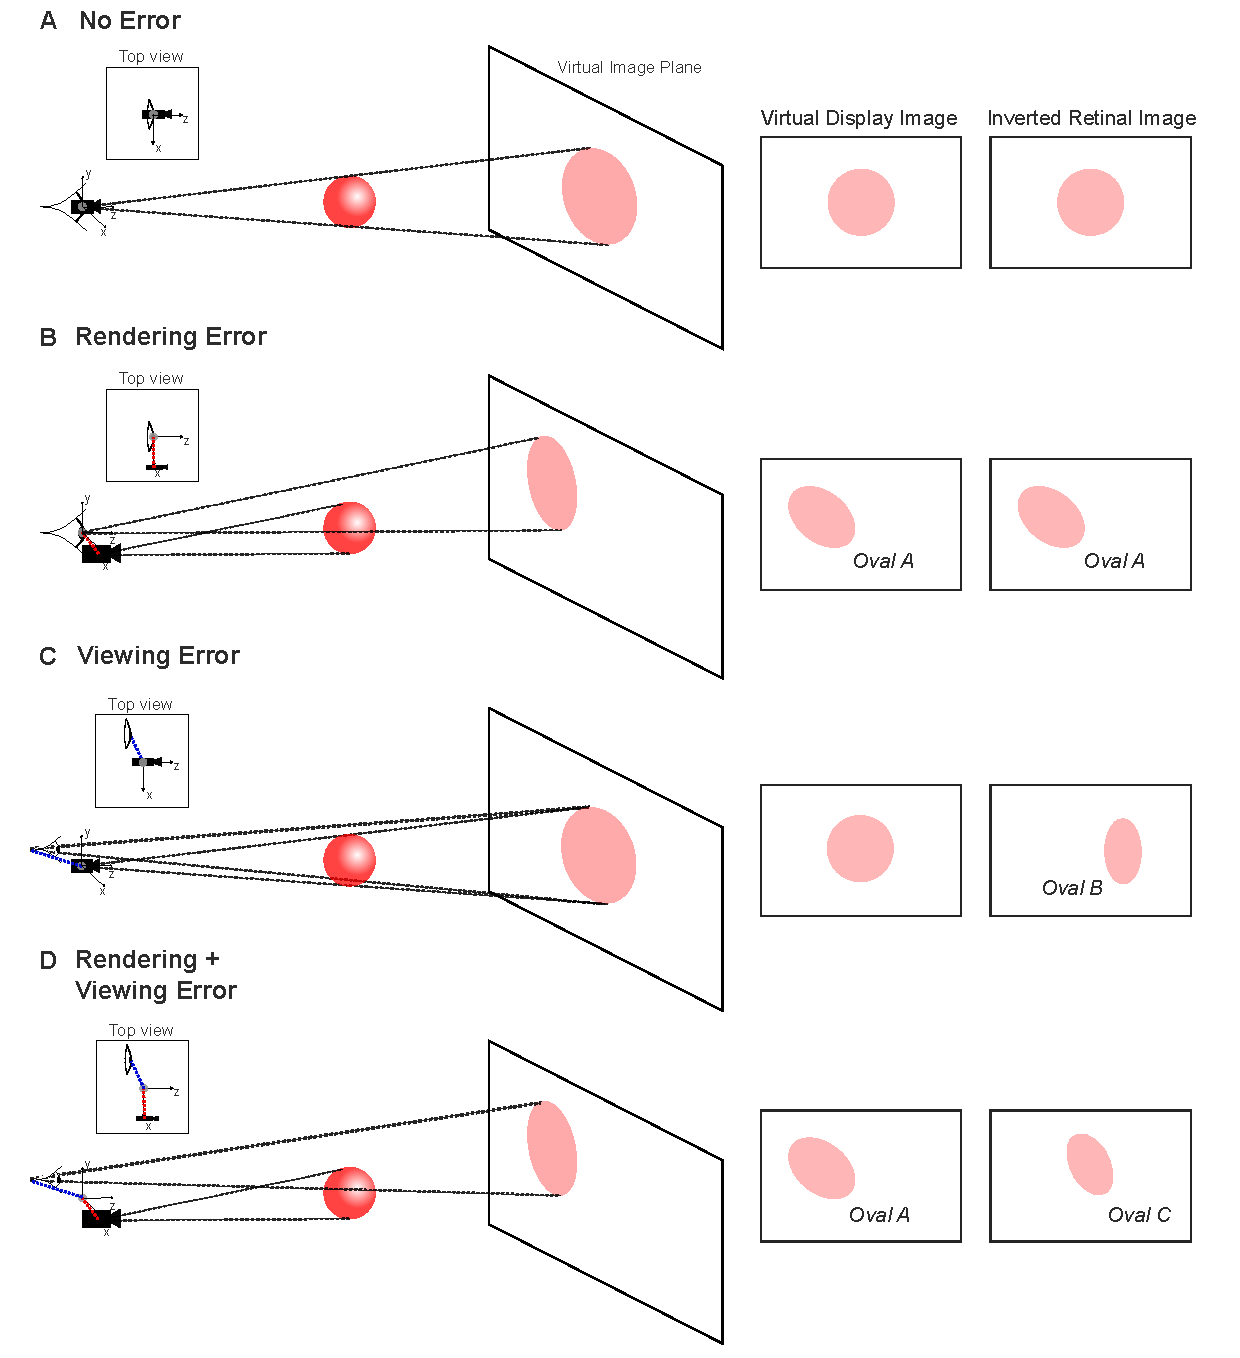
\includegraphics[width=\linewidth]{figures/model/rendering_vs_viewing_error.pdf}  
	     \caption{Comparing rendering error with viewing error (copied from main text). For simplicity, we show a monocular example as the set up is the same for both eyes. The origin of the coordinate system is at the HMD CoP (grey dot). The virtual sphere is positioned directly in front of the the HMD CoP. \textbf{(A)} In the ideal scenario, the render camera, CoP of the user's eye, and HMD CoP are all at the same position in space. No rendering or viewing error exists in this system. The camera is on-axis with the sphere and will render the corret perspective projection (a circle) that will be presented on virtual image plane. The user will view this circle from the intended CoP and the user's retinal image of what is shown on the display plane is also a circle. \textbf{(B)} The render camera is displaced to the right and down from the HMD CoP, creating a rendering error. The camera will render the sphere from this incorrect location, and render an oval instead of a circle. This oval is shown on the display plane and the user views it from the correct position so they perceive the same incorrectly rendered oval. \textbf{(C)} The CoP of the user's eye is displaced to the left and behind the HMD CoP, creating a viewing error. Despite the rendered image being correct on the virtual image plane, the perceived image is distorted. \textbf{(D)} In realistic usage, rendering and viewing errors typically occur together and can result in geometric errors being introduced in both render and viewing stages.}
	     \label{fig:rendering_vs_viewing_error}
	 \end{figure}


\paragraph{Rendering Errors}
The first step of an HMD render pipeline is to capture images, either from render cameras placed in a virtual scene, or from physical passthrough cameras on the HMD. We define rendering error as displacement of the render camera (or video passthrough camera) relative to the HMD CoP. For rendered content these errors generally arise from headtracking inaccuracy and user movement that moves the HMD CoP from the headset pose used for rendering (i.e., latency). Its impact is illustrated in Figure~\ref{fig:rendering_vs_viewing_error}B. Here the HMD CoP is on-axis with a sphere, but the render camera is not. Rays are captured by the render camera at an angle and the image presented on the display is an oval. The user views the display from the HMD CoP and perceives an oval rather than a circle which is the retinal image what a user would have seen if they had viewed a real sphere.

In video passthrough systems without view reprojection~\cite{ElChemalyGAP,kuo23} a static offset will exist between the cameras located at the front surface of the headset and the headset CoP. This type of passthrough error is similar to enlarging the user's head which will effectively exaggerate rotational head movement, corresponding to users viewing the world as if their heads were larger. Importantly, rendering errors affect parallax when user's move their heads, and objects closer to the rendering camera in a virtual scene are more affected by rendering errors compared to farther objects.

\paragraph{Viewing Errors}
Rendered or captured content is presented on the actual HMD displays from the left and right HMD CoP. These displays are very close to the user's eyes, and near-eye optics magnify these displays and move them to a comfortable virtual image distance, a process which requires optical distortion correction~\cite{robinett92, rolland93}. For simplification and generalizability we assume that the near-eye optics in HMDs are perfect lenses, and that images captured by the render camera can be simply projected onto a wide FOV plane at a virtual image distance (VID), typically between 1-2 meters away from the HMD CoP.

If the CoP of the user's eyes are not at the HMD CoPs then the images on the displays will not be perceived as intended. We define viewing error as displacement of the user eye CoP relative to the HMD CoP. An example of viewing error can occur if a user wears their own corrective glasses in an HMD which increases eye relief and place the user's eye too far away from the HMD CoP. In Figure~\ref{fig:rendering_vs_viewing_error}C the render camera is correctly located at the HMD CoP so the perspective image of the sphere is a circle. However, the user's eye is not at the HMD CoP so they see an oval instead. In this scenario the user's eye is off-axis to the sphere so they would see an oval in real life as well. However, the parallax shifts seen by the user during a viewing error is dependent on the virtual image distance, rather than the object distance. This underscores one of the important distinctions between rendering and viewing errors — objects very far away are marginally affected by rendering errors, but because the VID of an HMD is typically between 1-2 meters viewing errors can have large impacts on the perceived distance of these far objects.

\paragraph{Combined Rendering and Viewing Errors}
Figure~\ref{fig:rendering_vs_viewing_error}D shows the combined effect of these two types of viewing errors. Here a distortion from the target perspective projection of a circle is first introduced by the render camera being displaced from the HMD CoP. The oval that is shown on the display is additionally distorted from the user eye CoP being displaced from the HMD CoP, leading to an image of an oval on the retina that is different from the oval that was initially rendered. %Lastly, dynamic changes in the user's gaze will move user CoP (i.e., ocular parallax) and HMDs that do not account for ocular parallax will also cause a gaze-contingent viewing error \cite{lee2015effects, krajancich2020}. In the absence of rendering error, projected images on the virtual image plane of the display are geometrically correct however geometric errors will grow in magnitude as objects move farther away from the VID \cite{guan2023perceptual} (see supplementary materials).

\subsection{Coordinate Frame Transform of Reaching Data}

 Our participant reach data is recorded in the HMD coordinate frame and, for blind reaching, these distances must be transformed into egocentric coordinates to account for offsets between where the actual viewer's eyes are and where they are positioned in the HMD simulation platform. Table \ref{Entrance pupil relative to intended COP} shows the average displacement across all trials and subjects.


 \subsubsection{Egocentric Coordinates} \label{sec:ego_blind}

 We use the largest eye relief setting in the Quest 3 to accommodate the eyetracker added to the HMD. This results in an average eye relief that is 13 mm larger than expected (Table \ref{Entrance pupil relative to intended COP}, Z coordinate) and must also be accounted to interpret our measured reach as a user-perceived reach distance (Figure~\ref{fig:simulation_geometry}). This is accomplished by adding each individuals' eye relief error to the controller reach distance reported by the HMD. This transform is applied to all blind reaching conditions and this coordinate frame best represents how far away the target reach object appeared to the user.

 \subsubsection{Egocentric to HMD Coordinate Conversion} \label{sec:simulated_user_coords}

 In a typical HMD, egocentric reach distances cannot be measured without knowing both the actual user eye position and the nominal assumed user eye position. Thus, a more reliable measure of reaching performance is to instead consider reach distance in the HMD coordinate frame. In our HMD simulation platform, the IPD and passthrough error conditions do not displace the viewer and HMD origin. Therefore no additional transforms are necessary beyond compensation for the real eye relief errors described in Section~\ref{sec:ego_blind} to interpret the reaching results in HMD coordinates for IPD-IAD and passthrough errors. Eye relief viewing errors require an additional transform to account for the fact that the viewer's eye is not actually at the simulated position (Figure~\ref{fig:simulation_geometry}) and in our study this means an additional $\pm$3 cm shift to the egocentric blind reach distance. This coordinate system best represents the distance a user would reach to if the rendering and viewing errors simulated in our HMD platform were actually present in a real HMD instead of being simulated in our platform.

 %\subsubsection{Interpreting Sighted Reaching}

 %Regardless of the viewer's perceived target distance, they must reach to a distance that is 30 cm away from the headset to generate the same retinal images as the reaching stimulus (Figure~\ref{fig:simulation_geometry}). This means that, on average, participants must physically reach to 31.3 cm in order to perceive the controller at 30 cm (according to ray intersection geometry) in our baseline no-error condition.

\begin{table}[H]
	\centering
	\begin{tabular}{|c|c|c|c|}
		\hline
		& X (mm) & Y (mm) & Z (mm)\\
		\hline
		Left Eye & 1 $\pm$ 2 & 0 $\pm$ 3 & -13 $\pm$ 3\\
		\hline
		Right Eye & 0 $\pm$ 2 & 0 $\pm$ 3 & -13 $\pm$ 3\\
		\hline
	\end{tabular}
	\caption{Average entrance pupil position relative to the HMD COP of Quest 3. n = 6295 trials.}
	\label{Entrance pupil relative to intended COP}
\end{table}

\FloatBarrier
\begin{figure}[H]
	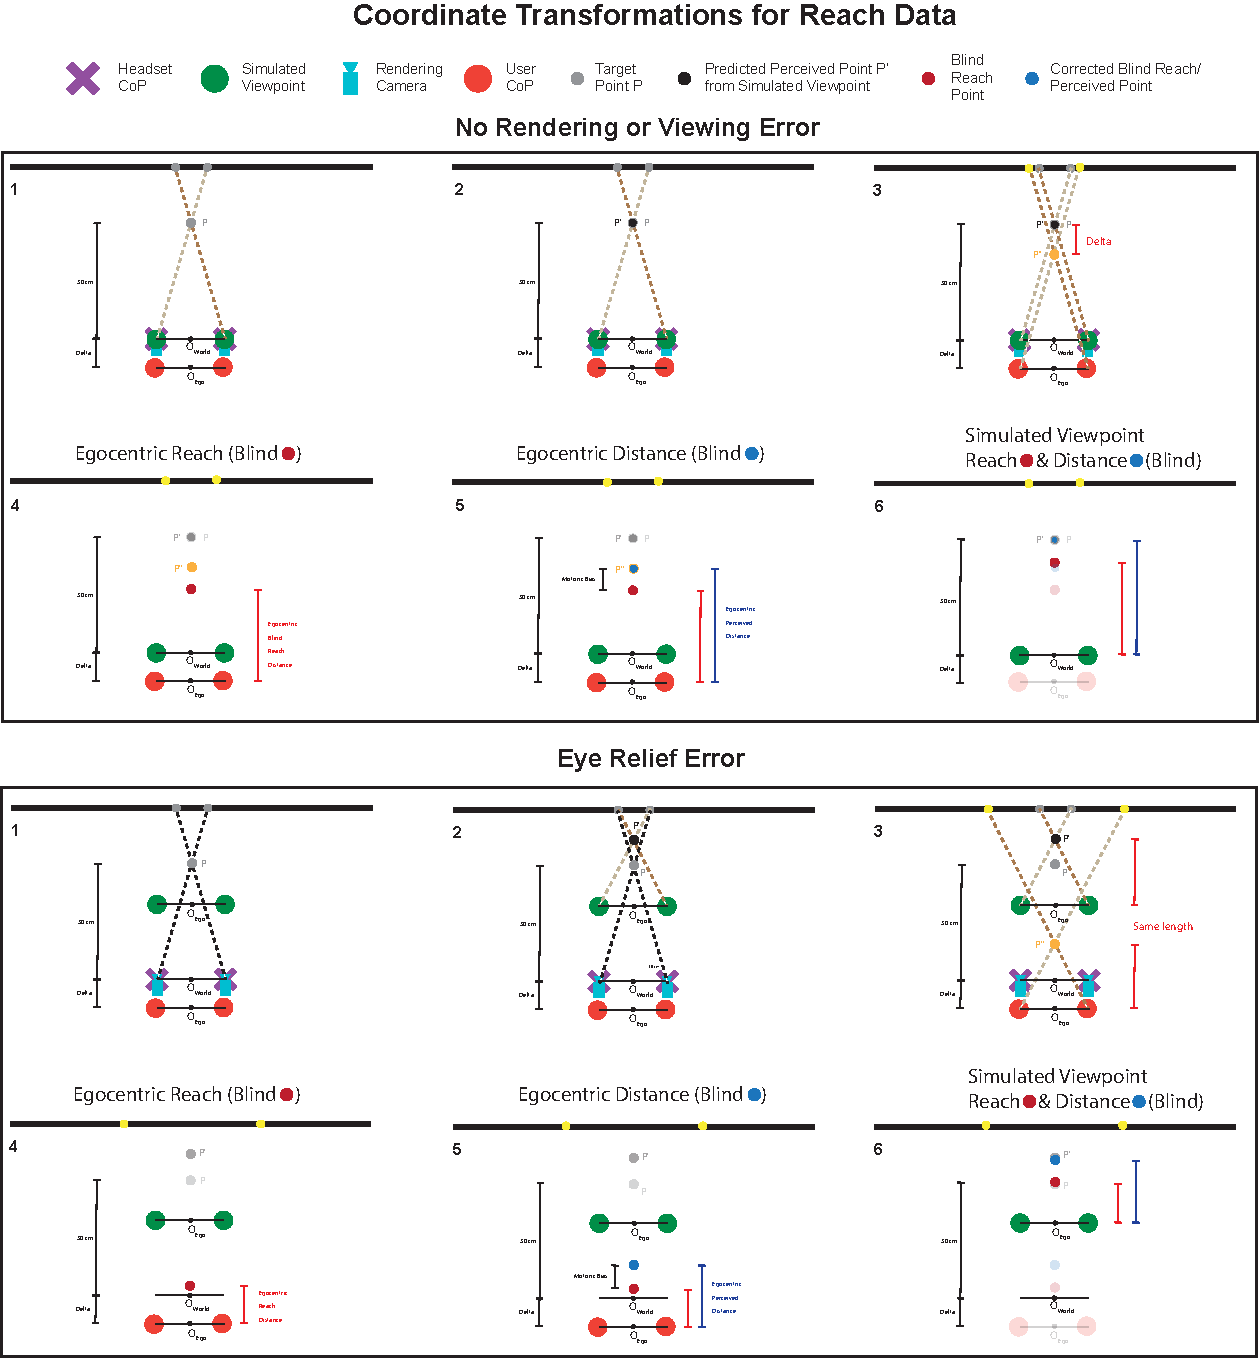
\includegraphics[width=\textwidth]{figures/supplement/world_vs_egocentric_frame_step_by_step_combined_no_sighted_reaching.pdf}
	\caption{Coordinate system transforms used to interpret reaching data studies. (Top) Our headset uses the largest Quest 3 eye relief setting available which
		results in an average eye relief viewing error of -12 mm. In panels 1-2, we show how a target point P is rendered at P’ when no stereo geometry errors are added
		to the system. In panel 3, the rays used to simulated viewpoint are shown to the actual user who is slightly displaced away from the ideal eye relief resulting in
		a perceived point P’. In panels 4-6, we describe how blind reaching and bias-corrected blind reaching can be converted from measured values into their equivalent perceived values based on the small offset delta between the actual user eye position and simulated viewpoint. (Bottom) Simulated eye relief viewing errors require another transform to interpret egocentric reach data in the simulated viewpoint world coordinates which is shown in panel 5 and 6. }
	\label{fig:simulation_geometry}
\end{figure}


\FloatBarrier


\subsection{Geometric Distortion Fields}
\mbox{}

\begin{figure}[h]
	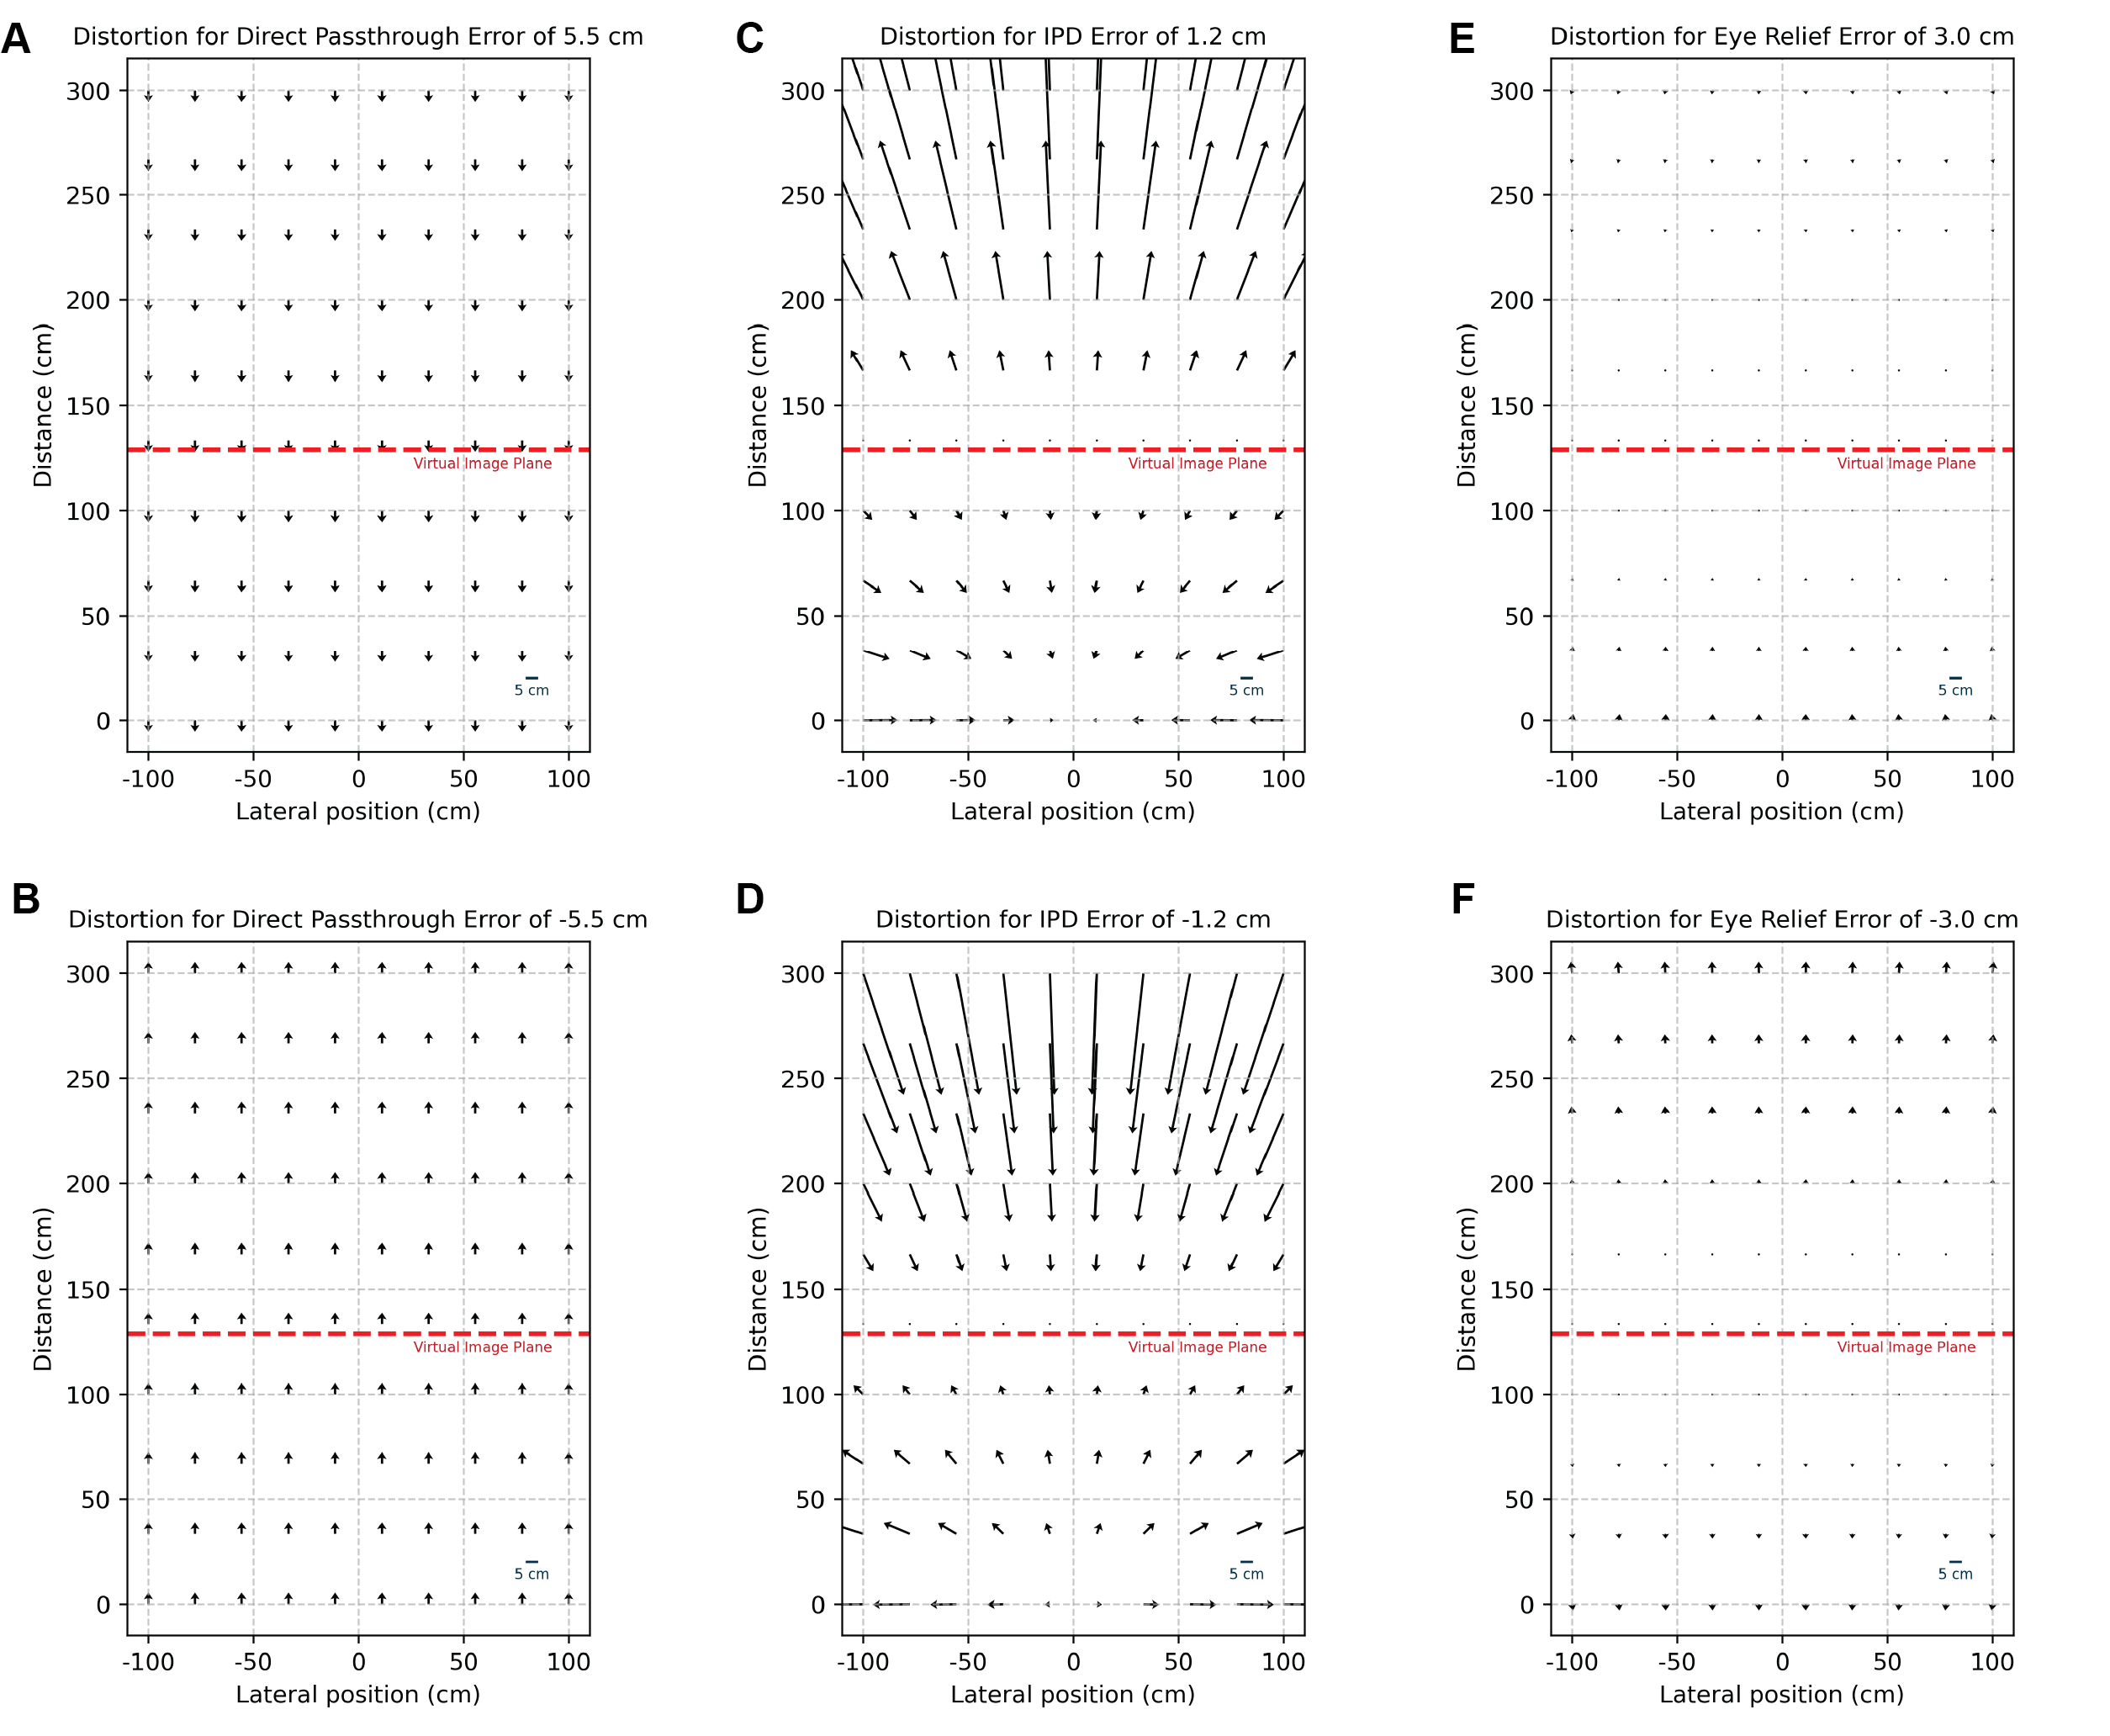
\includegraphics[width=\textwidth]{figures/supplement/suppl_distortion_field.png}
	\caption{Geometric distortion fields in HMD coordinates at errors used in reaching experiments. (A,B) Direct Passthrough errors. (C,D) IPD Error. (E,F) Eye
		Relief Error. For viewing errors (C-F), points on the virtual image plane are not distorted. For rendering errors (A-B), distortions are the same irrespective of
		virtual image plane distance. Ocular parallax is on for panels A and B to visualize the effect of rendering error only.}
	\label{fig:suppl_distortion_field}
\end{figure}


\FloatBarrier
\newpage
\section{Experiment 1}
\subsection{Reaching Experiments Supersubject Raw Data}

\begin{figure}[h]
	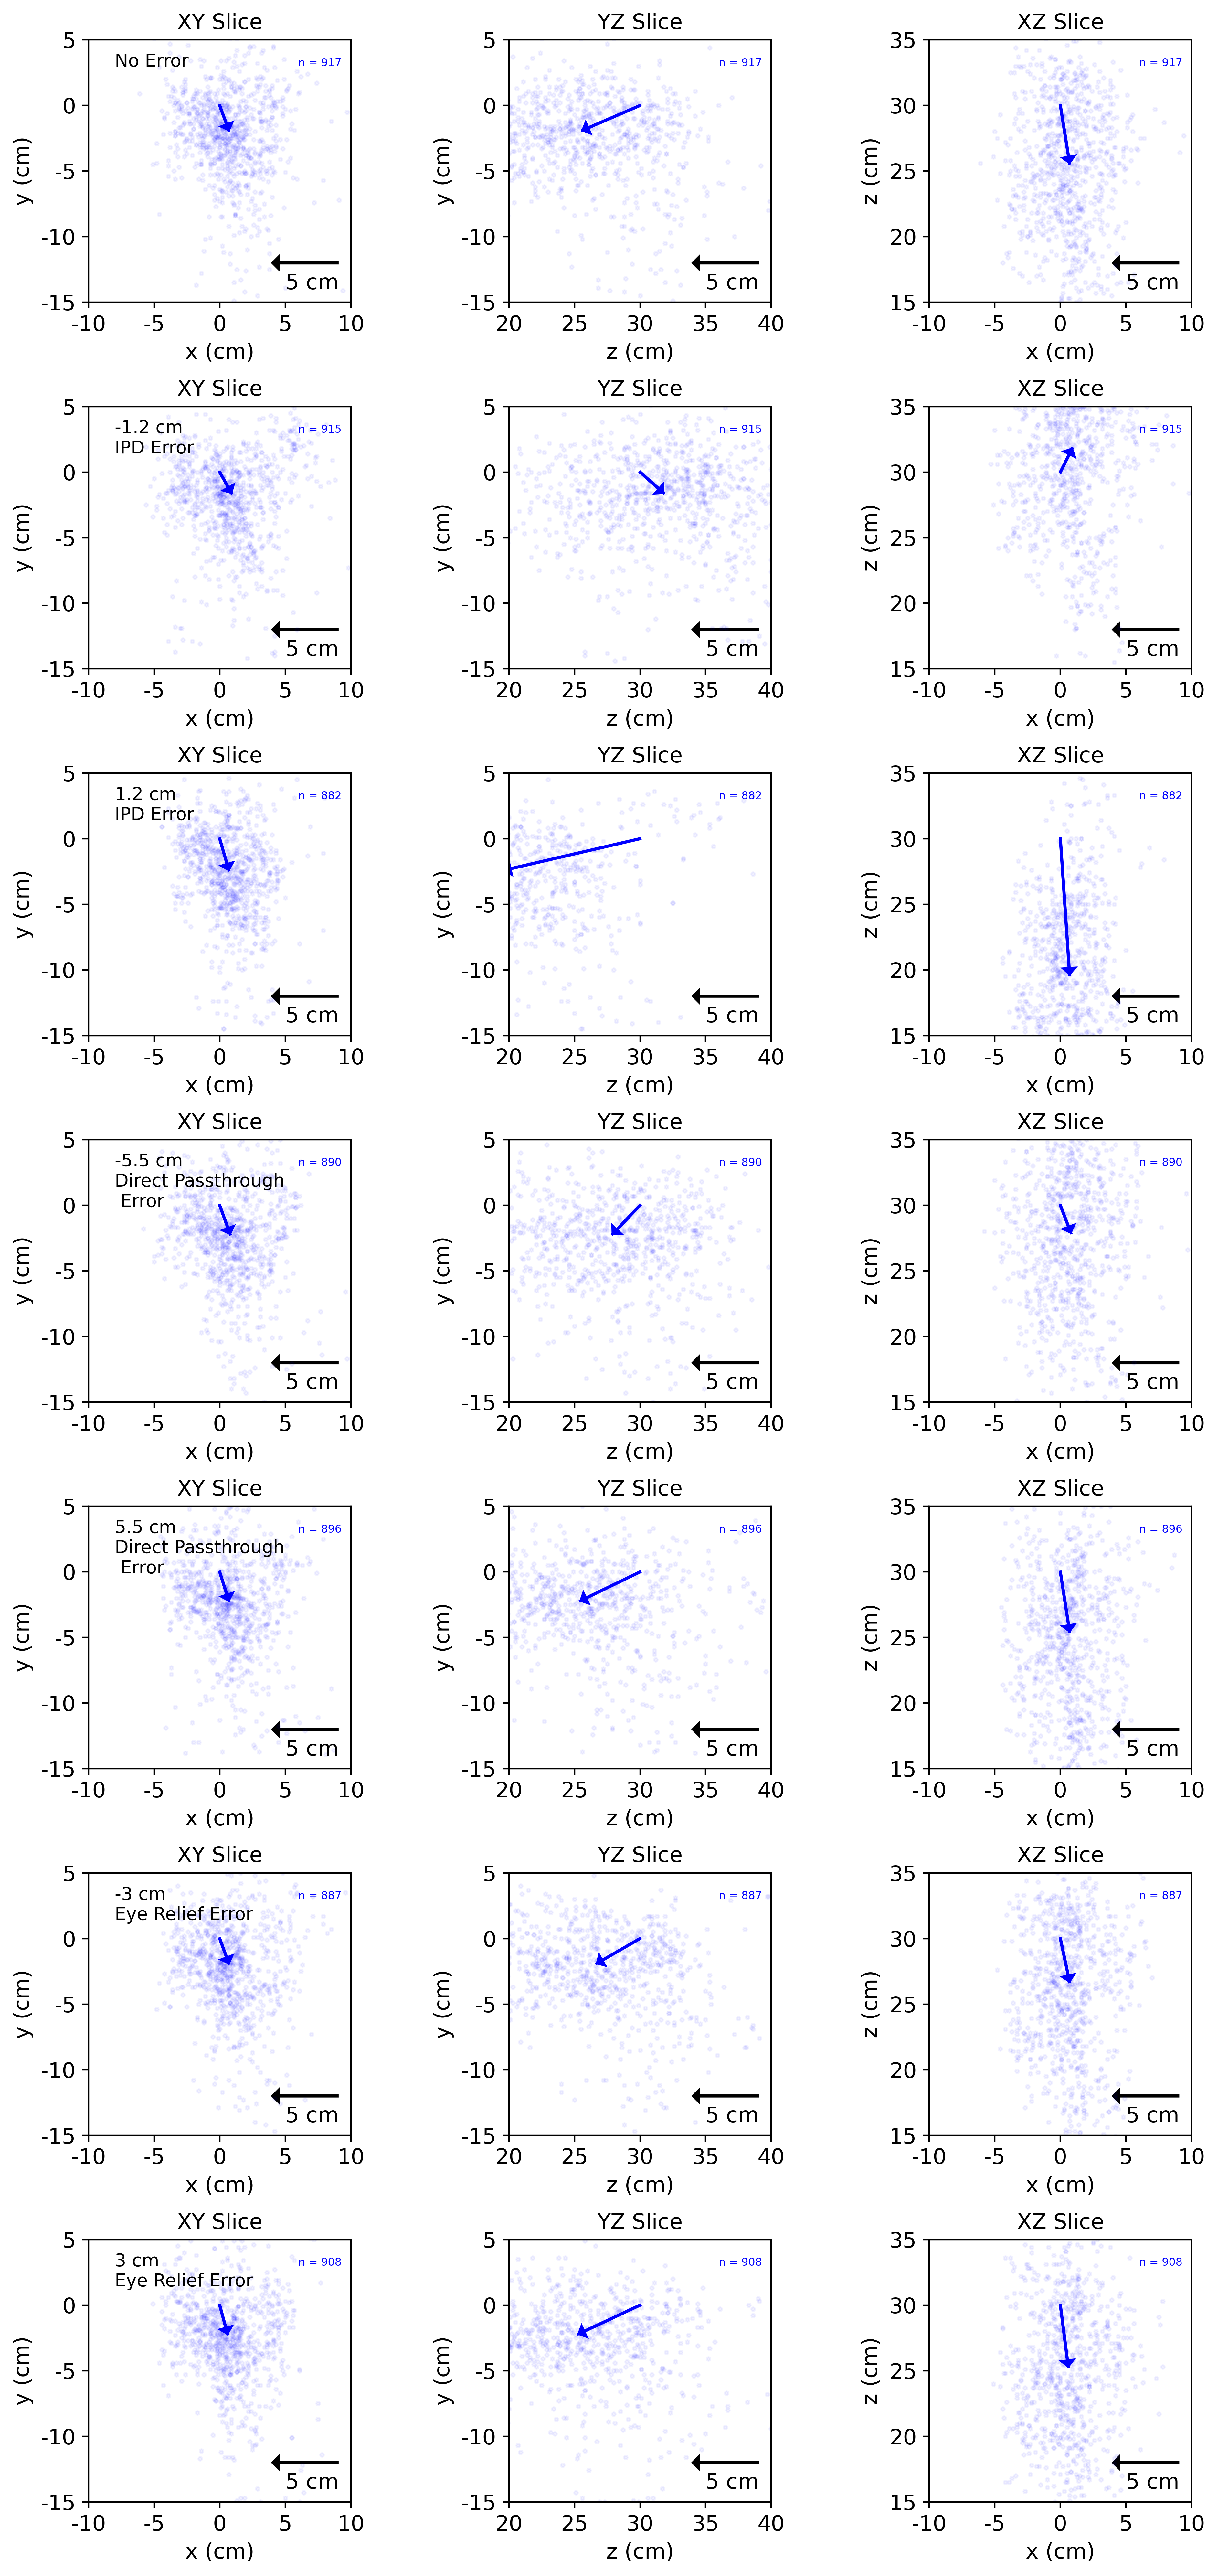
\includegraphics[width=0.47\textwidth]{figures/supplement/super_subject_raw_data.png}
	\caption{Raw recorded reach positions across all 32 participants. Each row represents the same data projected onto different planes, visualizing from the front (XY slice), side (YZ slice), and top (XZ slice). Each dot is a single participant's reach. Arrowhead coordinates are determined from the medians of x, y, z reach positions separately. The coordinate system is left handed. Physically, positive x, y, z, correspond to the right, top, and front of the user, respectively.}
	\label{fig:super_subject_raw_data}
\end{figure}

\FloatBarrier
\newpage

\subsection{Reaching Experiments One Example Subject Data}

\begin{figure}[h]
	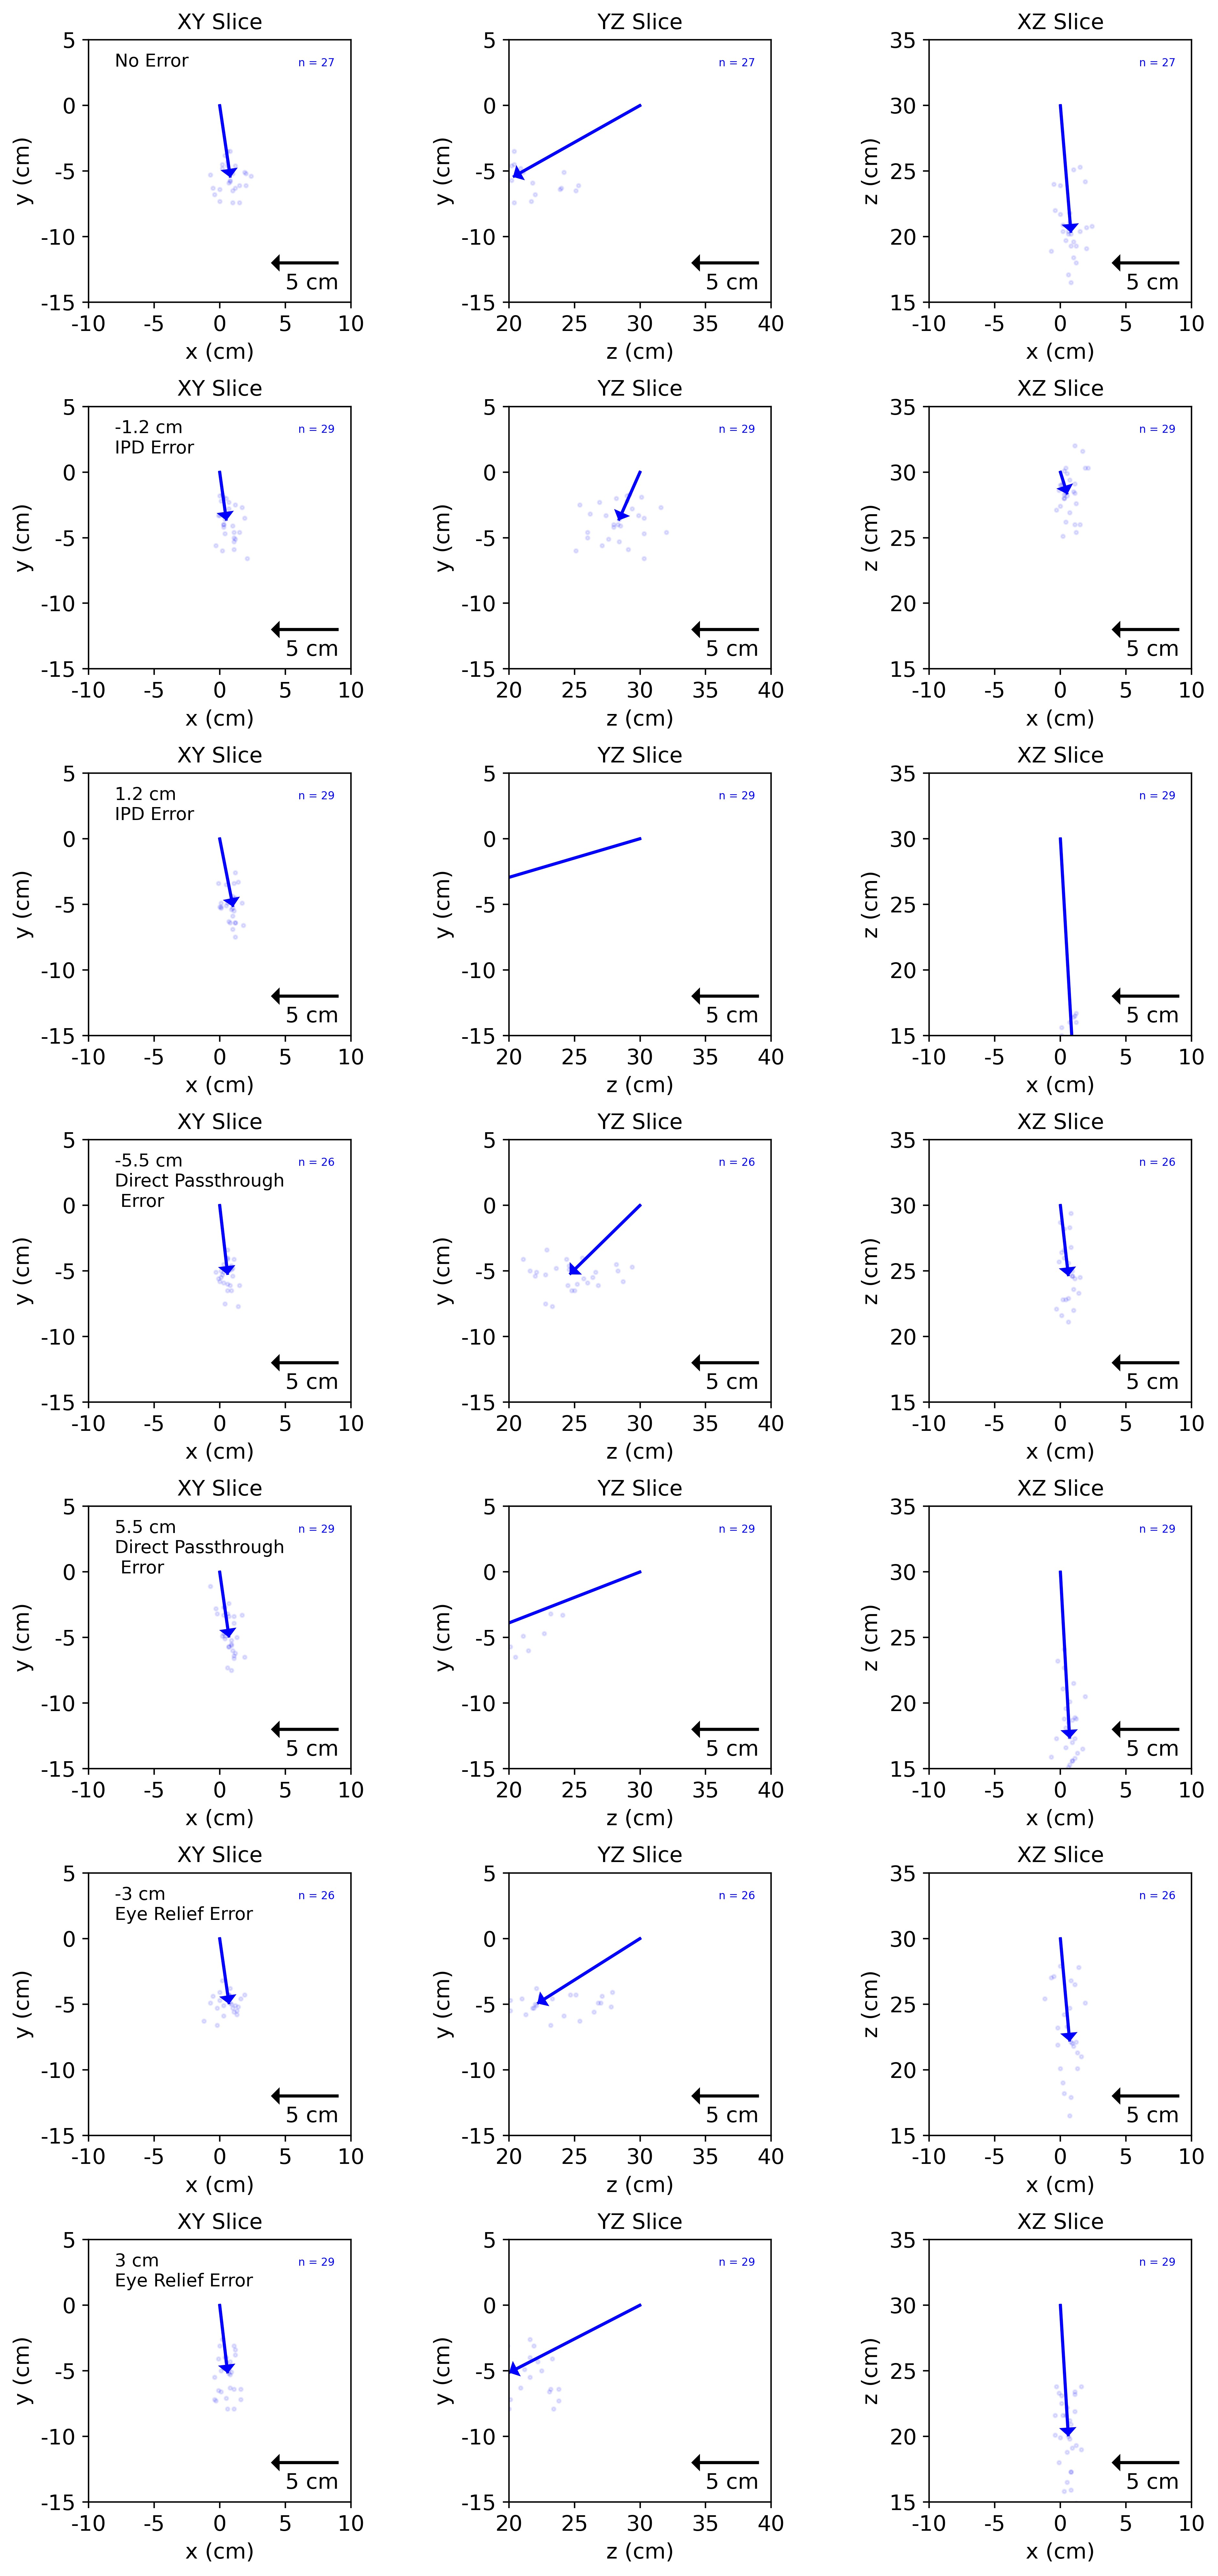
\includegraphics[width=0.47\textwidth]{figures/supplement/subject_14_raw_data.png}
	\caption{Raw recorded reach positions for a single participant. The XZ Slice of No Error condition is shown in Figure 1B of the main text. }
	\label{fig:subject_14_raw_data}
\end{figure}

\FloatBarrier
\newpage

\section{Experiment 2}
\subsection{Geometric Model Predictions}
Geometric simulations of IPD viewing error predict that the perceived distance exhibits significantly different behavior based on the target object's distance relative to the VID. If the object is in front of the VID, then the perceived object distance will be farther than intended when the HMD IAD is smaller than the user IPD (Figure~\ref{fig:model_predictions}B,C). If the object is behind the VID, then the same error will lead to the perceived object distance be closer than the intended distance (Figure~\ref{fig:model_predictions}B,E). If the object is at the VID exactly, then IAD and IPD mismatches should have minimal impact on the object's perceived distance (Figure~\ref{fig:model_predictions}B,D). For direct passthrough rendering error, we do not expect this behavior. A positive error (render camera in front of HMD CoP) make the stimulus appear closer at all three distances (Figure~\ref{fig:model_predictions}A,C-E). Our analysis in Section \ref{sec:slope} shows the direct of misperception in the human data are consistent with this geometric model. Crucially, we see the magnitude of distance perception is much larger for IPD error than direct passthrough error at 0.5 m and 2.5 m based on stereo geometry.


\begin{figure}[H]
	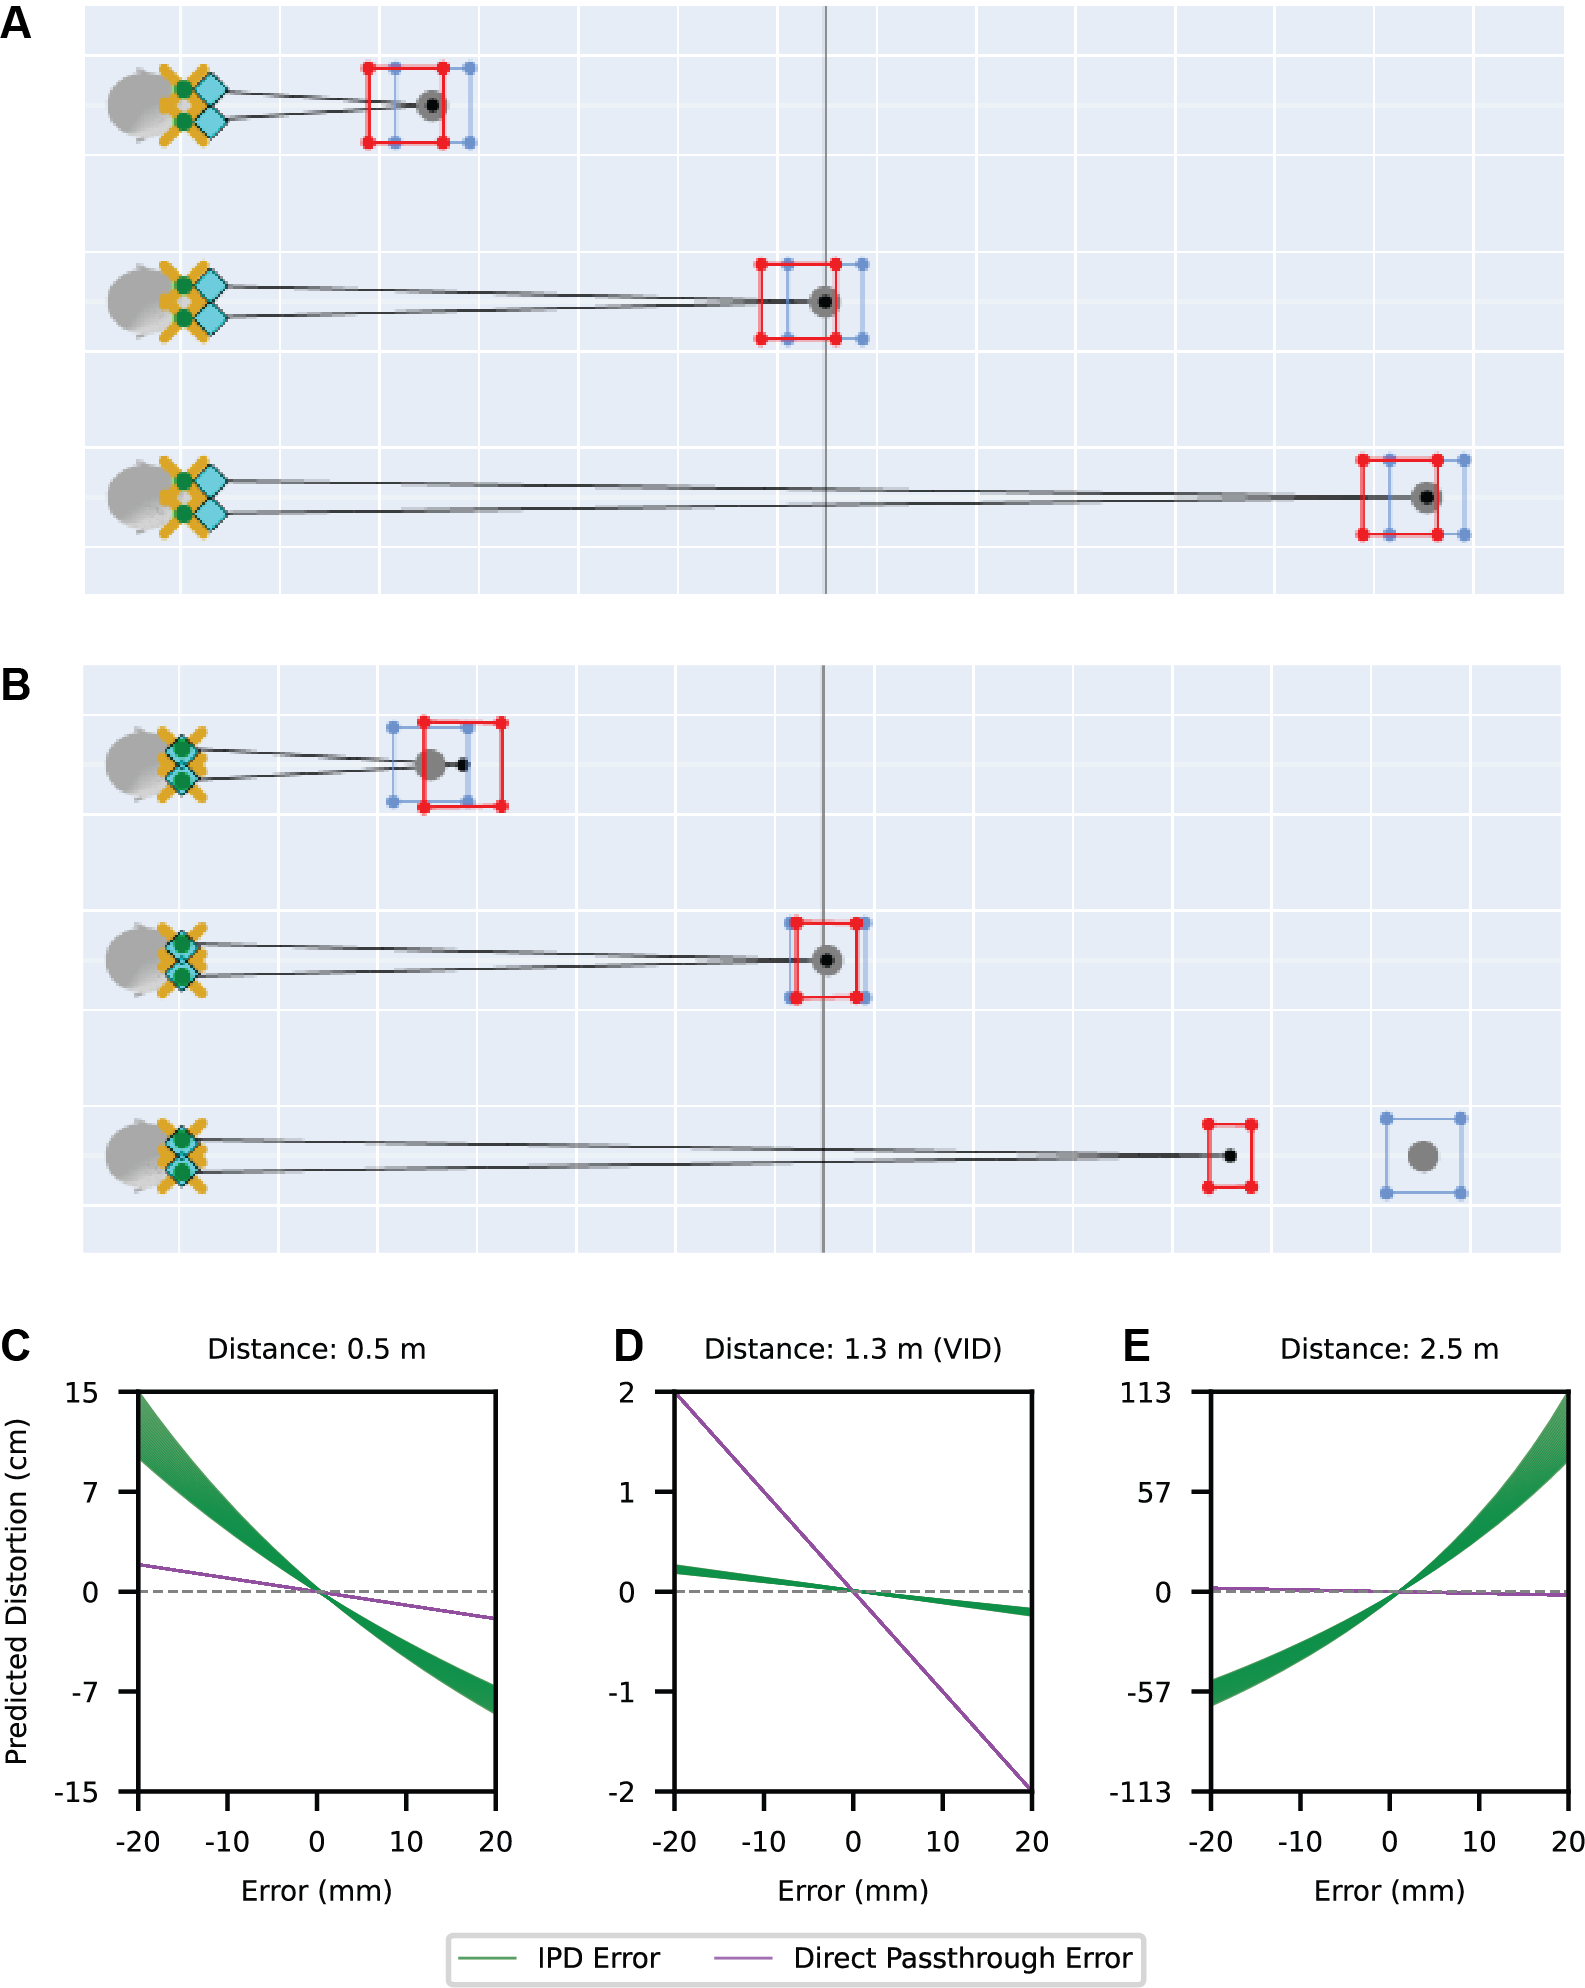
\includegraphics[width=.5\linewidth]{figures/visual/model_predictions.png}
	\caption{Distance misperception in relation to virtual image distance (VID). \textbf{(A)} and \textbf{(B)} show triangulation model predictions for a direct passthrough rendering error of +5.5 cm (render cameras in front of HMD CoP) and IPD viewing error of -1.2 cm (HMD IAD smaller than user IPD) for target distances at 0.5, 1.3 (VID), and 2.5 meters. The target boundary is shown in blue and the perceived boundary in is shown in red. \textbf{(C)}-\textbf{(E)} Distance misperception as a function of error magnitudes for user IPDs ranging from 55 mm to 75 mm. A negative value means the object is perceived as closer.}
	\label{fig:model_predictions}
\end{figure}

\FloatBarrier

\subsection{Psychometric Fitting}
The psychometric function we used is the logistic function:

\begin{equation}
	P_C = \gamma+(1- \lambda - \gamma) \cdot \frac{1}{1 + e^{-s(x - \alpha)}}
	\label{eqn:logistic}
\end{equation}

% \begin{description}
	%     \item[$\gamma$:] Guess rate
	%     \item[$\lambda$:] Lapse rate
	%     \item[$s$:] Slope
	%     \item[$x$:] Error
	%     \item[$\alpha$:] Threshold
	% \end{description}

The lapse rate $\lambda$ and guess rate $\gamma$ were set to 0.01 and 0 respectively. Threshold $\alpha$ and slope $s$ were the free parameters. We used the $minimize$ function of the $optimize$ module from the Scipy library in Python to perform a Maximum Likelihood Estimation on the binary response data \cite{KINGDOM201655}. We minimized the negative log likelihood of data given the model:

{\small
\begin{equation}
    \log(L) = \sum_{x} \left[ n_C(x) \cdot \log(P_C(x)) + (n_T(x) - n_C(x)) \cdot \log(1 - P_C(x)) \right]
    \label{eqn:loglikelihood}
\end{equation}
}
where $P_C$ is given by Equation \ref{eqn:logistic}, and $n_T$ and $n_C$ are respectively the total number of trials and the number of correct trials for a stimulus level. We bootstrapped the raw data and refit the function 200 times for each participant to obtain a distribution of the fitted threshold parameter. We found the bootstrapped threshold distributions were well behaved with no extreme values. 
\newpage

\subsection{Supersubject Psychometric Function for Error Detection: IPD Error}
\mbox{}
\begin{figure}[H]
	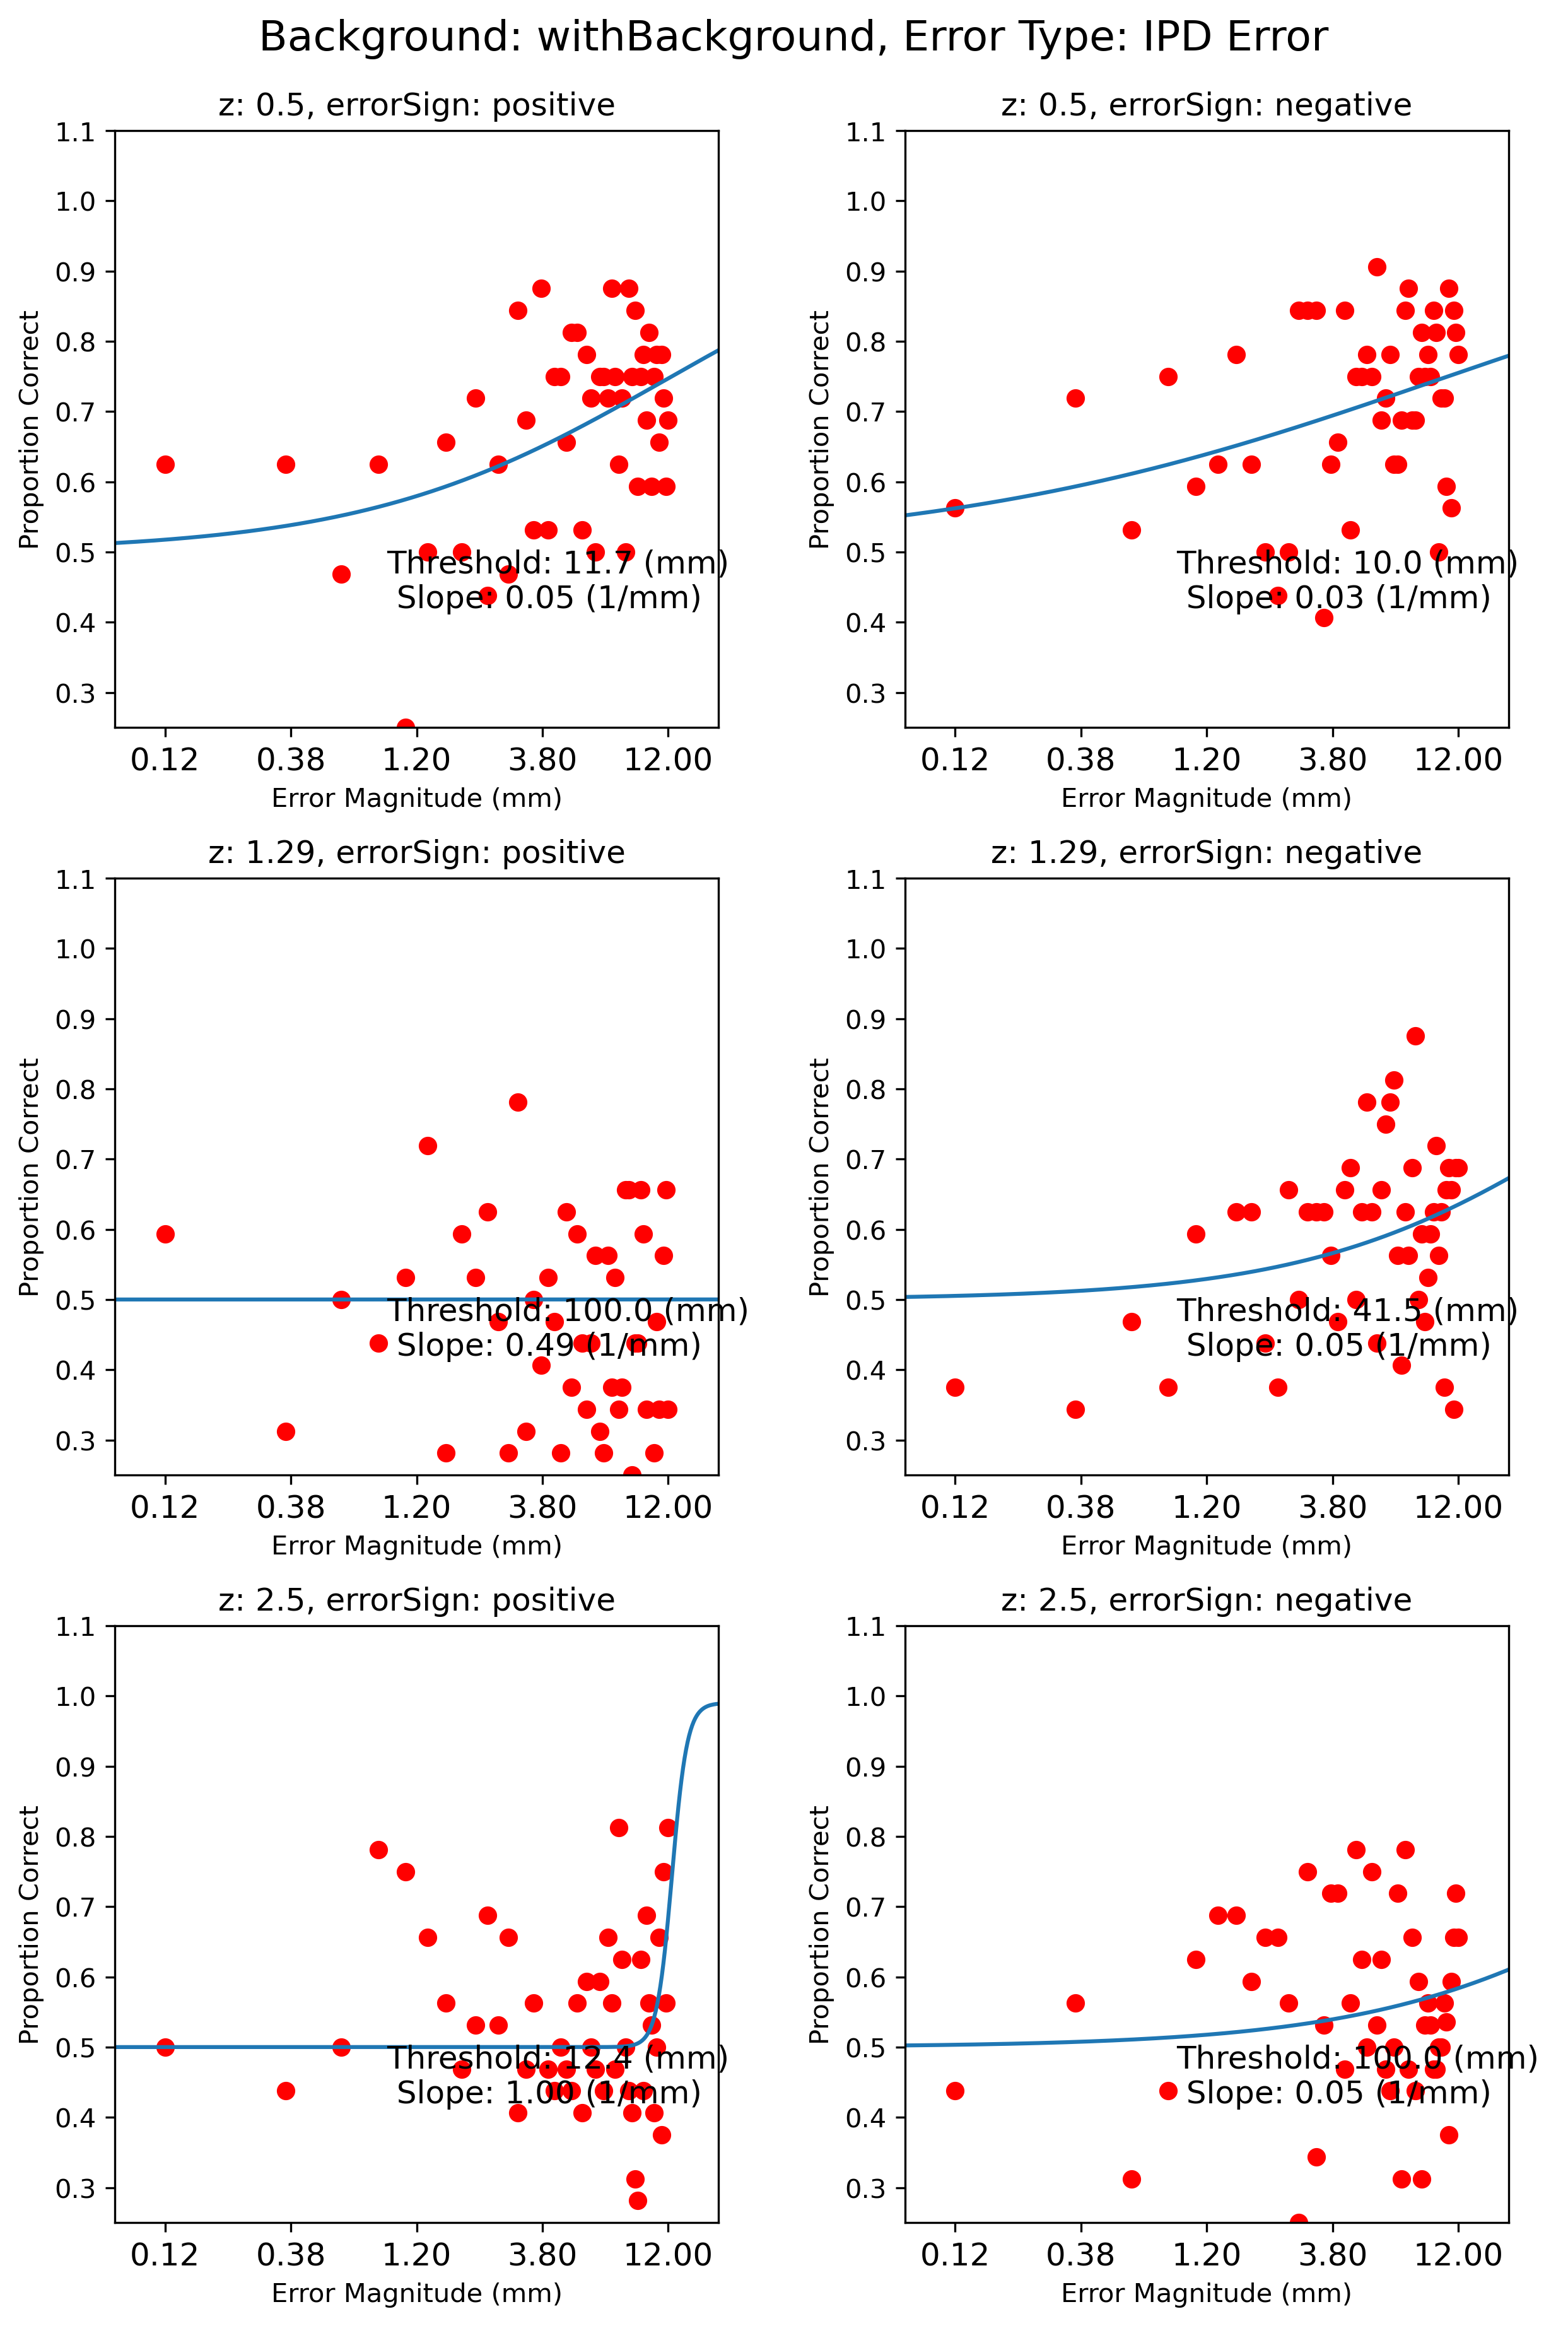
\includegraphics[width=.65\textwidth]{figures/supplement/visual_only_experiment_super_subject_fits_withBackground_IPDError.png}
	\caption{Psychometric function of best fit on the combined data across all 32 participants for IPD error. Top row: 0.5 m. Middle row: 1.3 m. Bottom row: 2.5 m. Left column: positive error. Right column: negative error. Each red point represents the probability of detection, calculated from responses from 32 participants for that error level. The psychometric function is fit to the raw binary data.}
	\label{fig:visual_only_experiment_super_subject_fits_withBackground_IPDError}
\end{figure}

\FloatBarrier
\newpage

\subsection{Supersubject Psychometric Function for Error Detection: Direct Passthrough Error}
\mbox{}
\begin{figure}[H]
	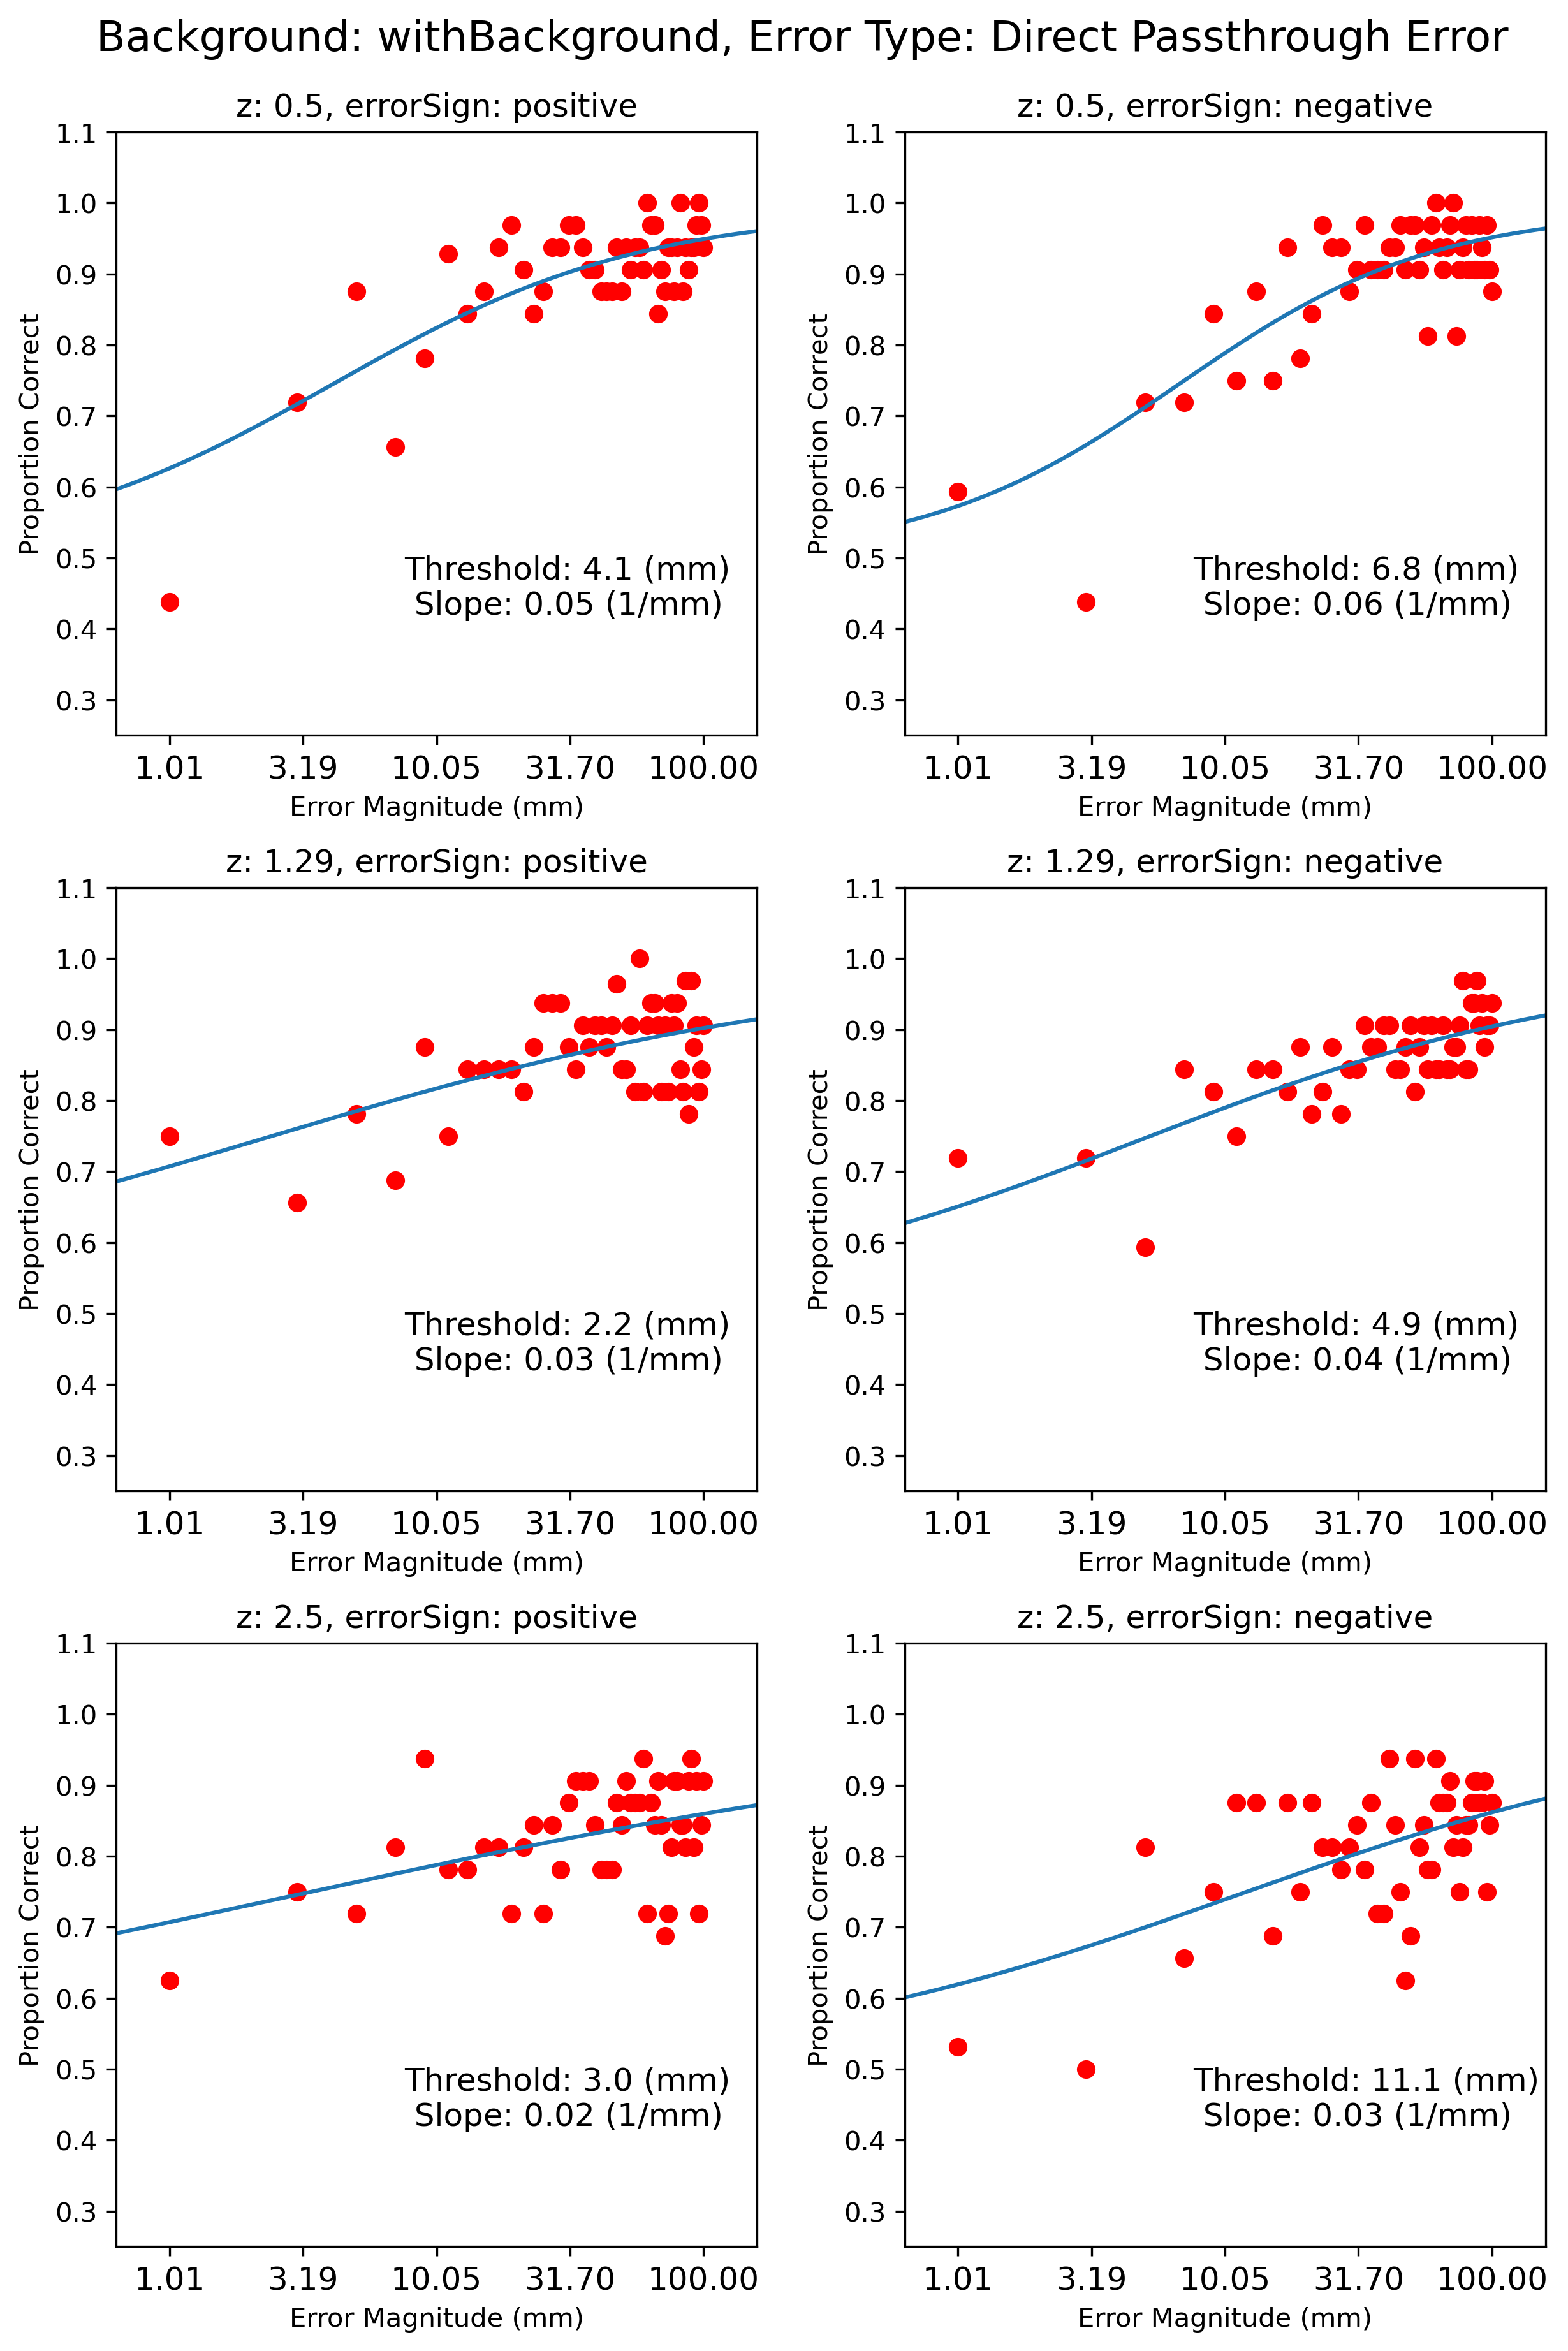
\includegraphics[width=.65\textwidth]{figures/supplement/visual_only_experiment_super_subject_fits_withBackground_zRenderingError.png}
	\caption{Psychometric function of best fit on the combined data across all 32 participants for direct passthrough error.}
	\label{fig:visual_only_experiment_super_subject_fits_withBackground_zRenderingError}
\end{figure}

\FloatBarrier
\newpage

\subsection{Example Participant Psychometric Function for Error Detection: IPD Error}
\mbox{}
\begin{figure}[h]
	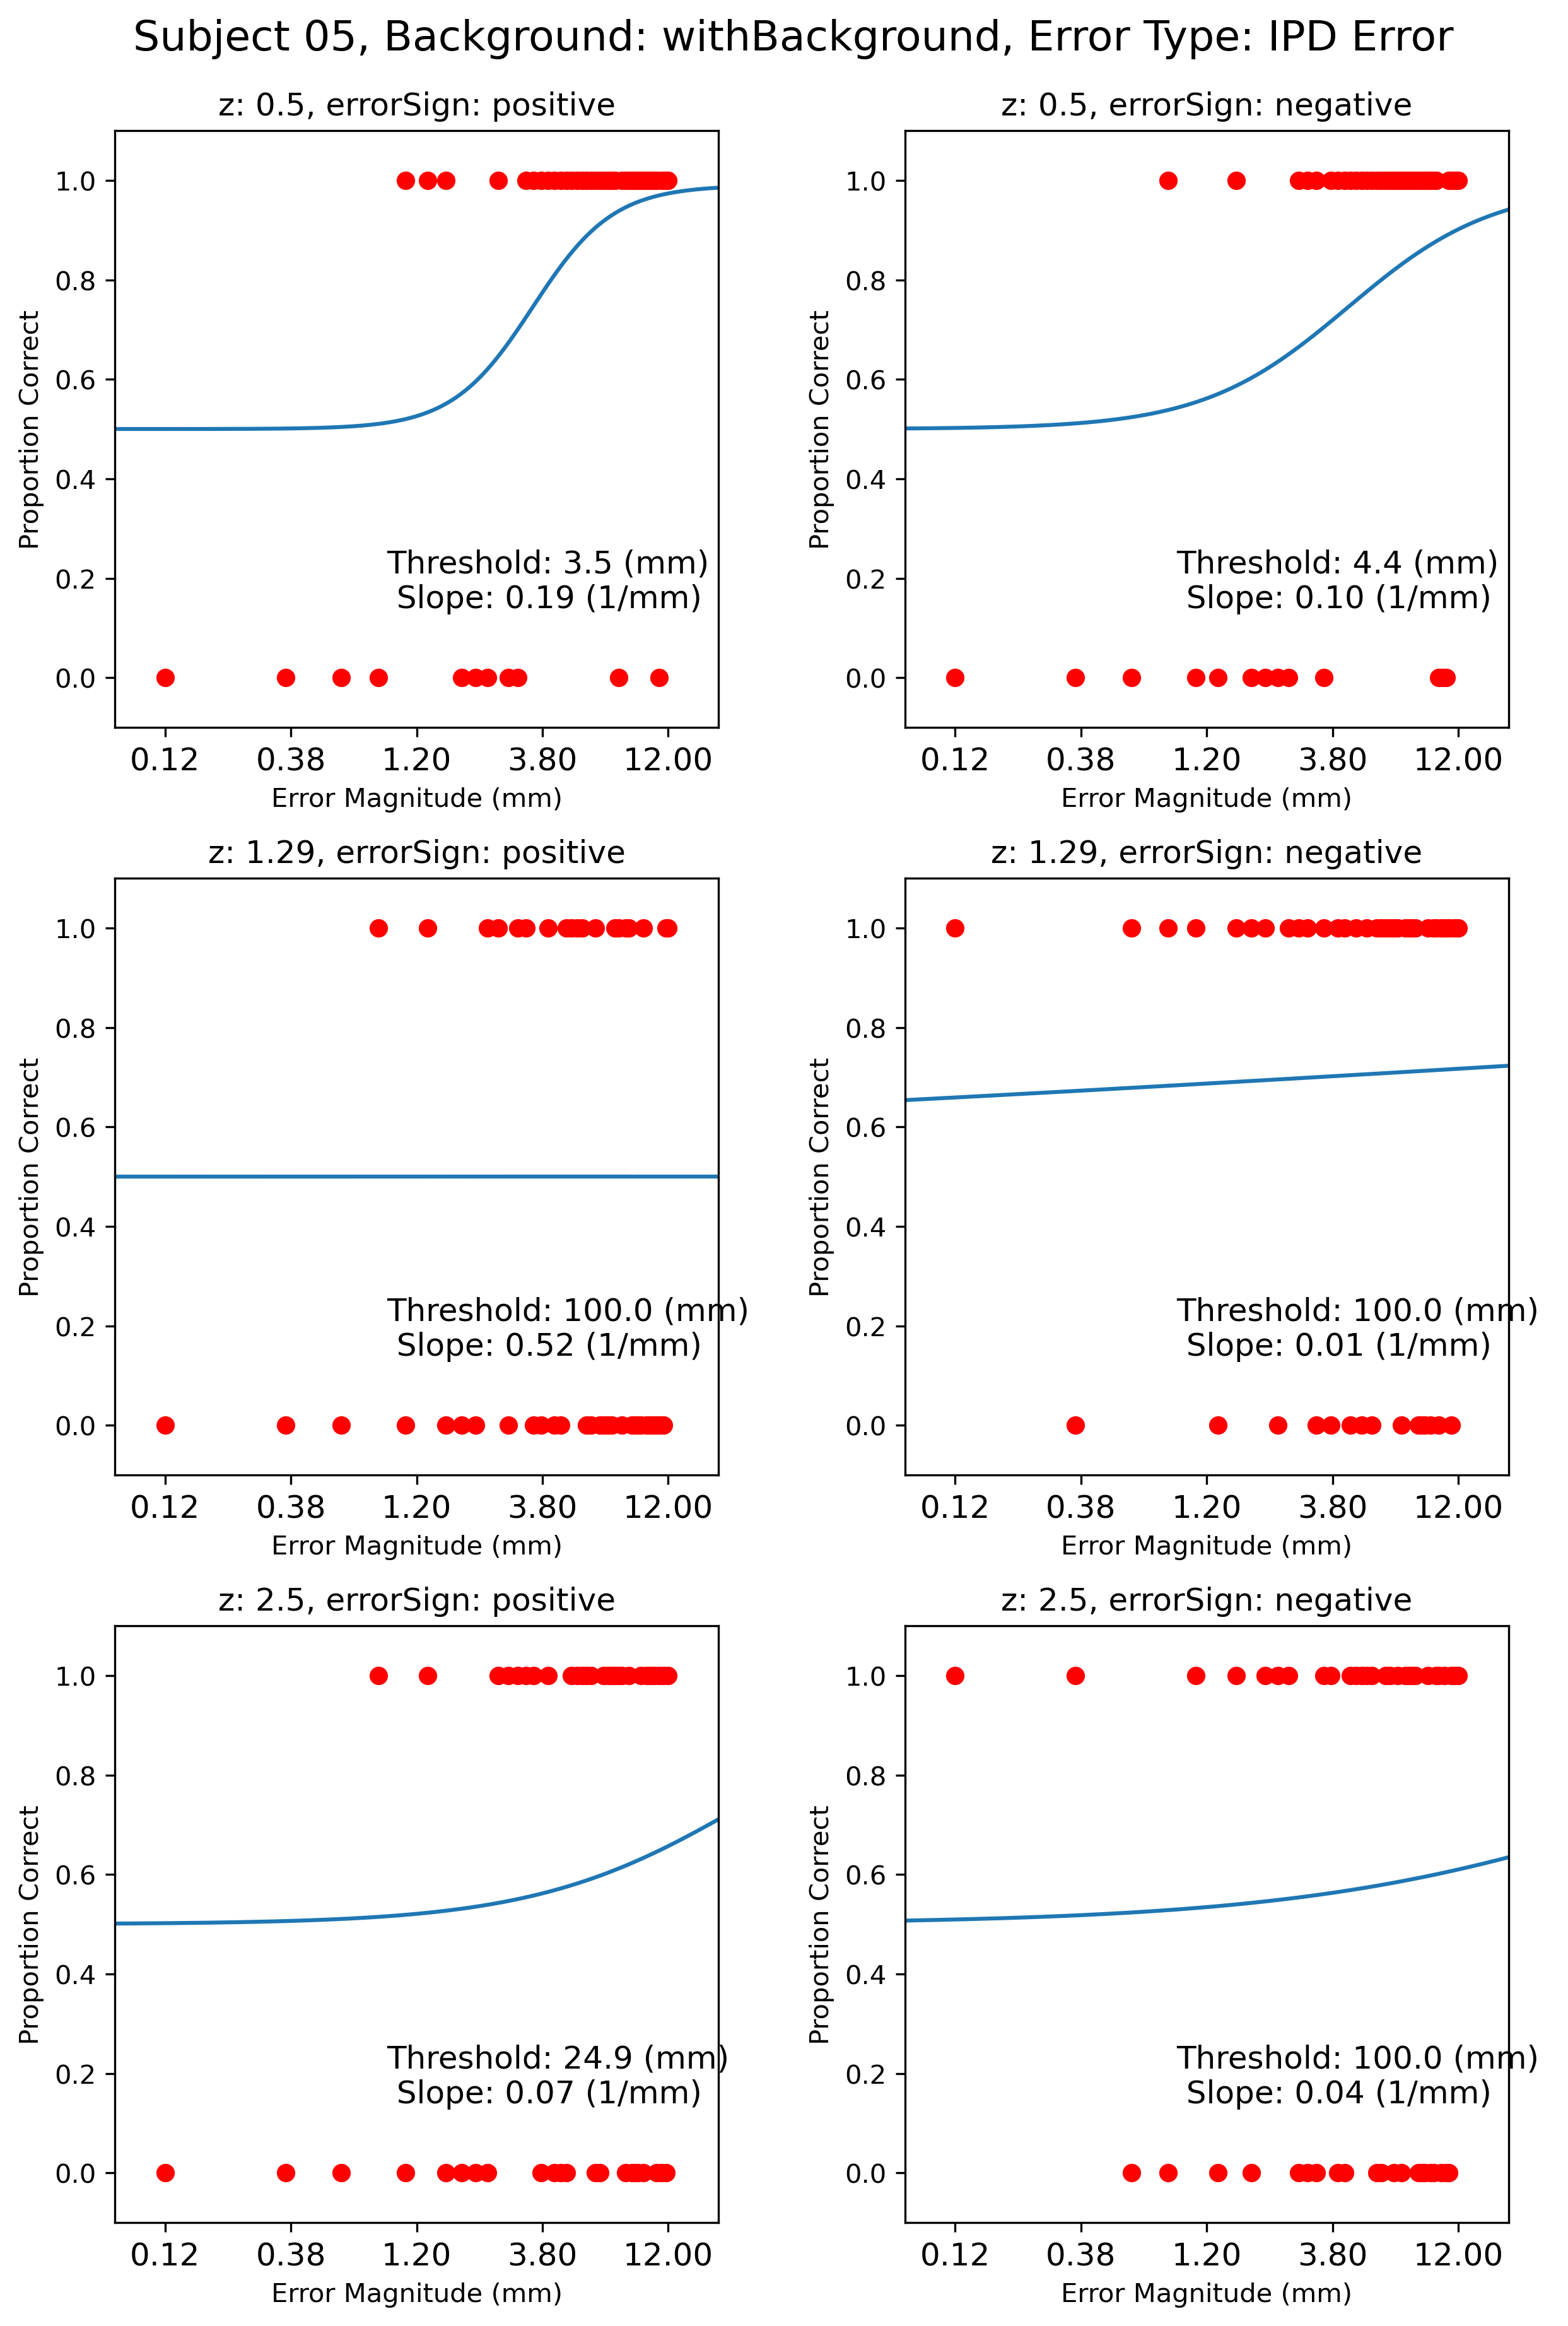
\includegraphics[width=.65\textwidth]{figures/supplement/visual_only_experiment_subject_05_fits_withBackground_IPDError.png}
	\caption{Psychometric function of best fit for a single participant for IPD error. The top left panel is shown in Figure 1C of the main text. }
	\label{fig:visual_only_experiment_subject_05_fits_withBackground_IPDError}
\end{figure}

\FloatBarrier
\newpage

\subsection{Example Participant Psychometric Function for Error Detection: Direct Passthrough Error}
\mbox{}
\begin{figure}[h]
	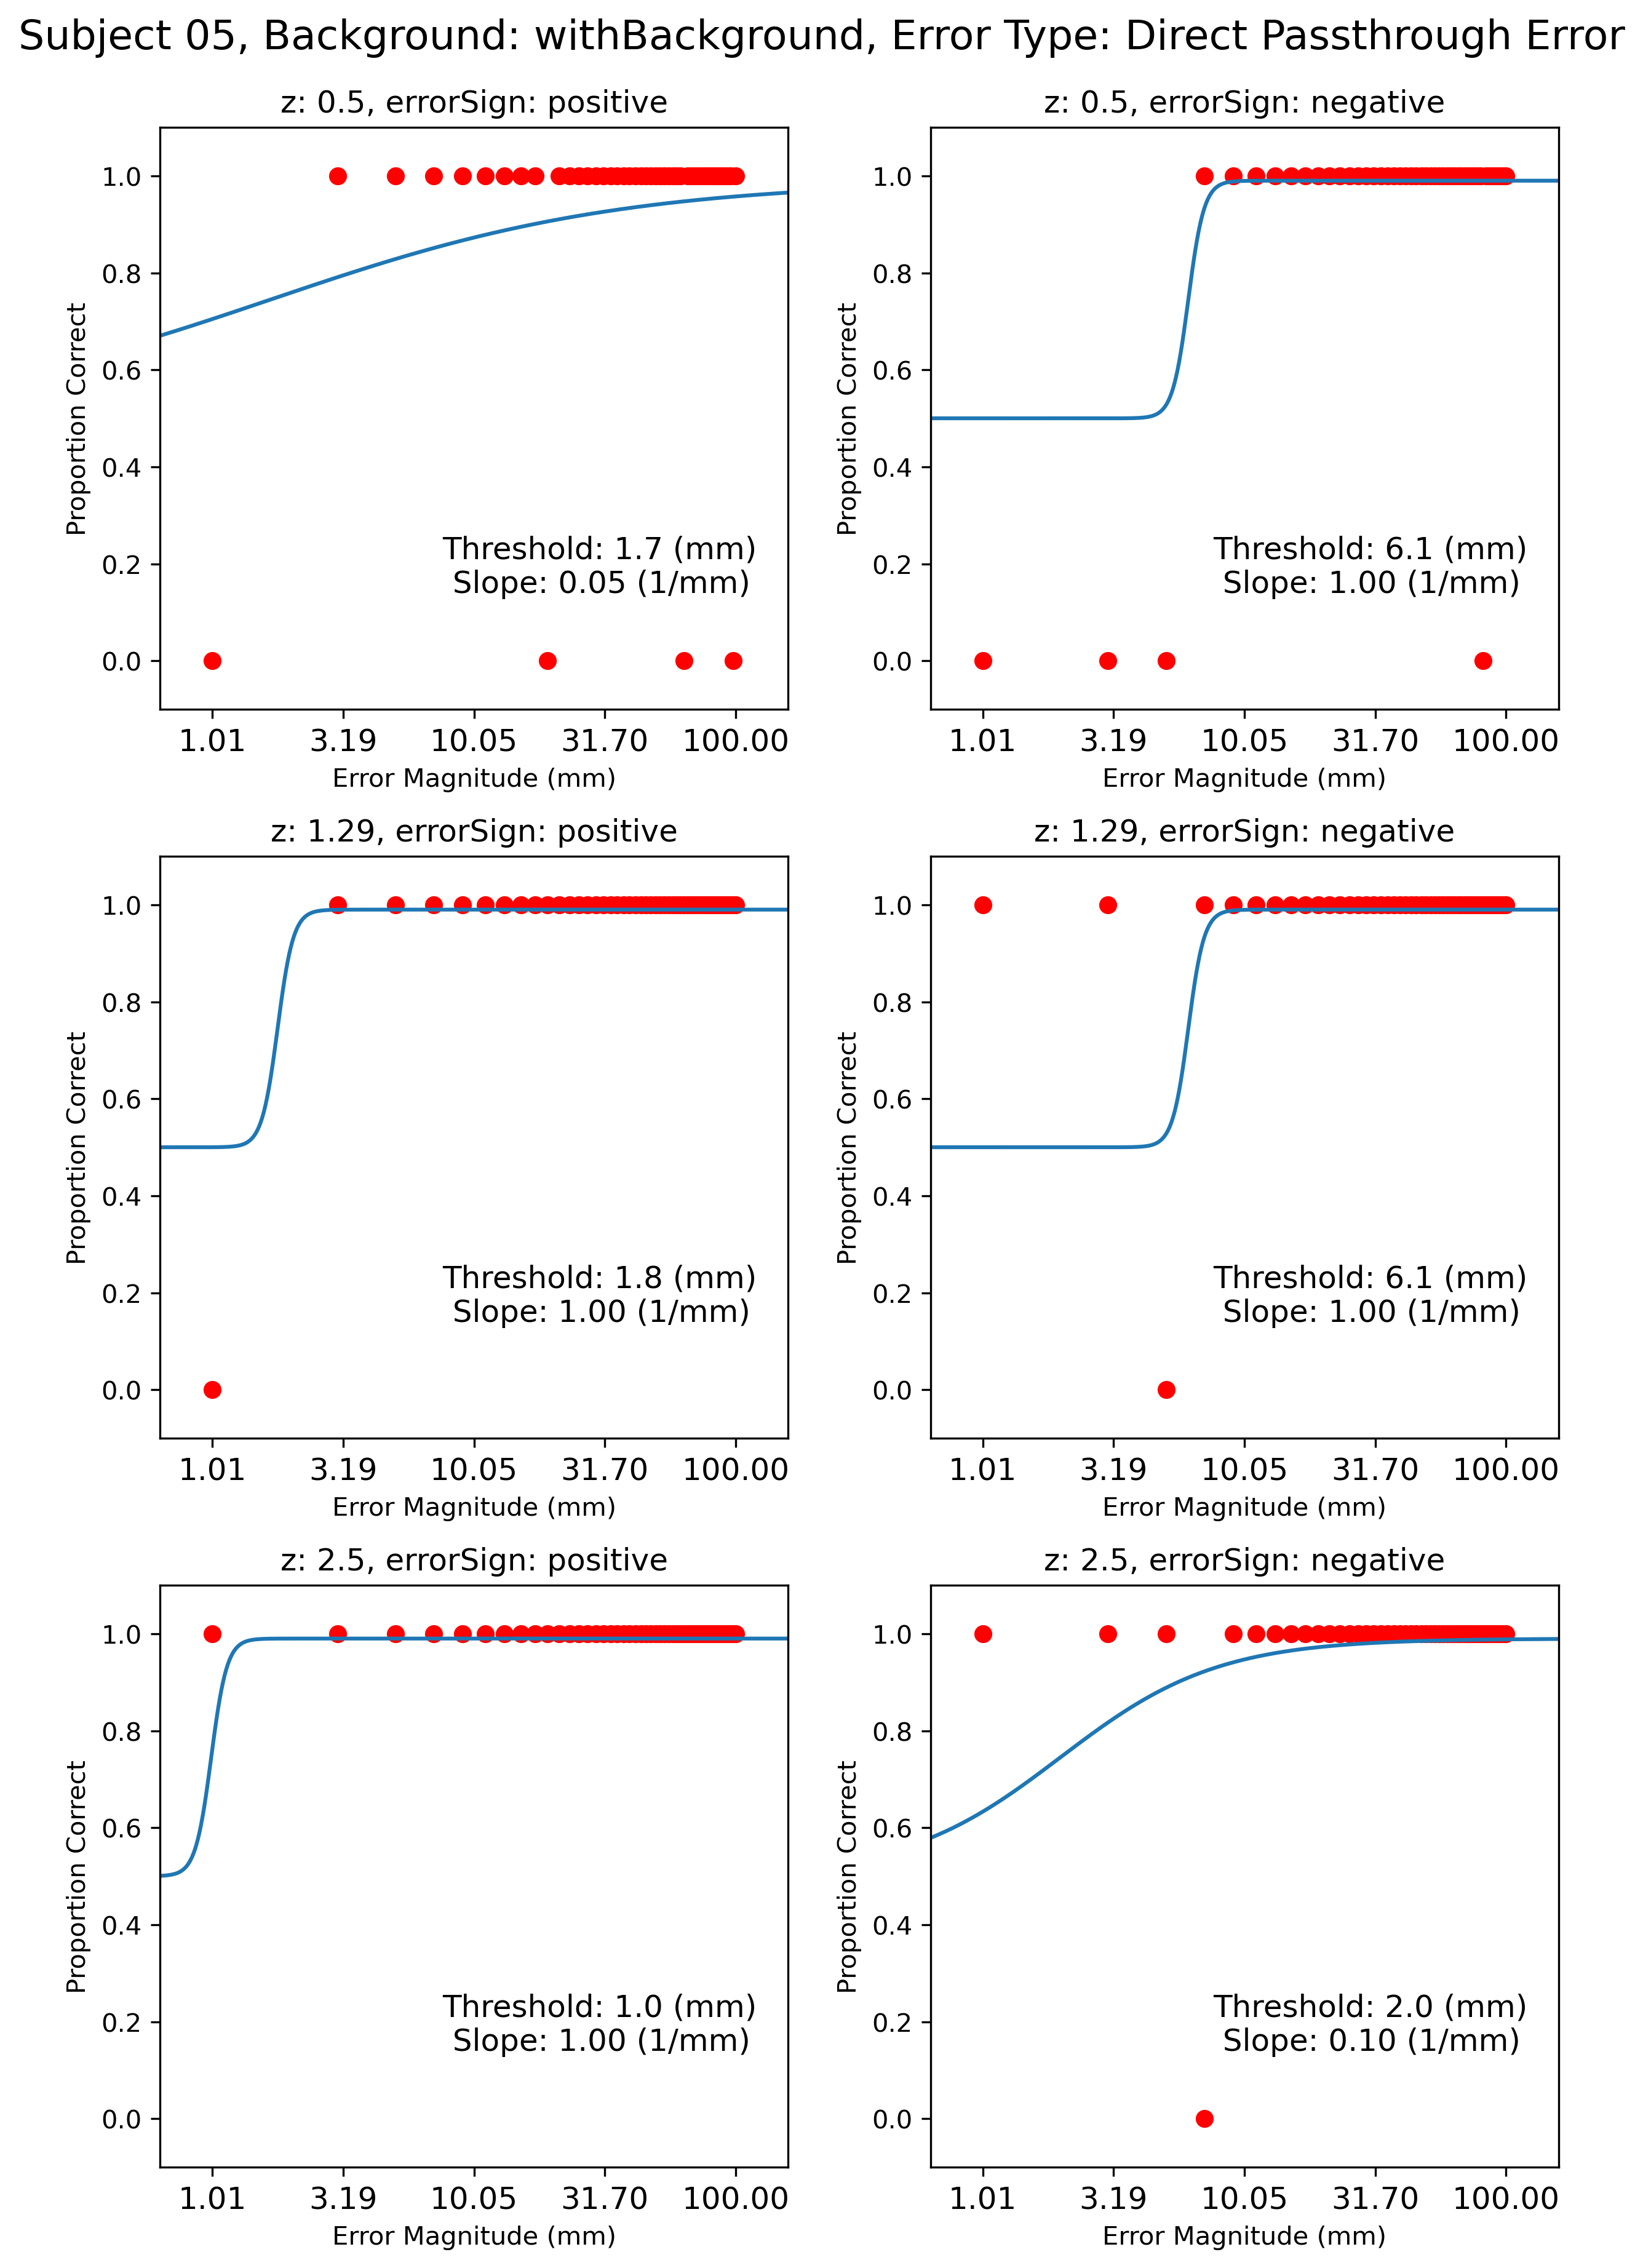
\includegraphics[width=.65\textwidth]{figures/supplement/visual_only_experiment_subject_05_fits_withBackground_zRenderingError.png}
	\caption{Psychometric function of best fit for a single participant for direct passthrough error. }
	\label{fig:visual_only_experiment_subject_05_fits_withBackground_zRenderingError}
\end{figure}

\FloatBarrier

\subsection{Psychometric Slope Analysis} \label{sec:slope}
\mbox{}
To more explicitly demonstrate the change in direction of distance misperception, we carried out an additional analysis investigating the direction and sensitivity of perceived distance. This was achieved by fitting the same psychometric function described in Section~\ref{sec:slope} to both positive and negative error data with slope as the only free parameter with threshold $\alpha$ fixed to 0. The sign of the slope indicates how adding error affects the target's perceived distance, and its magnitude indicates the participant's sensitivity to that specific error. 

We specified a maximal model linear mixed effects model to evaluate the impact of viewing distance on each participant's sensitivity to changes in passthrough rendering errors or IPD viewing errors. The maximal model in for this analysis is:  
\begin{equation}
	\text{slope} \sim \text{distance} + (\text{distance} | \text{ID})
\end{equation}
where slope was the best-fit slope of a single participant's psychometric function and distance was the distance of the visual target.

\begin{figure}[H]
	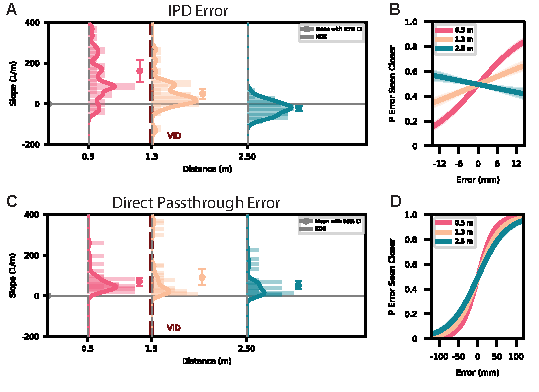
\includegraphics[width=0.9\textwidth]{figures/supplement/slope_summary.pdf}
	\caption{Slope analysis of visual perception experiment. Panels \textbf{(A)} and \textbf{(C)} show the slope parameter values as a function of distances (0.5, 1.3, and 2.5m) for IPD error and direct passthrough error respectively. Panels \textbf{(B)} and \textbf{(D)} show the "supersubject" psychometric functions for IPD error and direct passthrough error respectively. n=32.}
	\label{fig:slope_summary}
\end{figure}

 \subsubsection{IPD Error}
The slopes of psychometric functions fit on the combined data of all thirty-two participants (a "super subject") are shown in Figure~\ref{fig:slope_summary}B and slopes for each individual are shown in Figure~\ref{fig:slope_summary}A. At the group level, the slope did change sign for the near and far object distances (linear model estimate: -32.34 at 2.5 meters), which means that the same IPD manipulation has the opposite effect on perceived distance as predicted by the geometric model. The model predicts a zero slope when the target is at 1.3~m; we do not find a flat slope here, but we do find that the slope is flatter for the 1.3~m target compared to the 0.5~m target with more participants having psychometric functions with positive, but smaller slopes (Figure~\ref{fig:slope_summary}A). There is a clear effect where the psychometric function slope declines across the three distances (main effect of distance: $\beta$ = -88.998; t = -6.32; p < 0.0001; intercept: $\beta$ = 190.16; t = 6.20; p < 0.0001). The slopes of these functions are similar to the direct passthrough rendering errors, but appear shallower in the figures because we were limited by the range of IPD errors that could be simulated before changes in vergence demand became too significant across trials, thus the range of the IPD viewing error figures are approximately one order of magnitude narrower. 

Since the psychometric function slope does become negative at 2.5 meters (linear model estimate: -32.34), it is likely that a target probe placed somewhere between 1.3 to 2.5 meters would result in a nearly flat psychometric function.One possible reason for this observed discrepancy is that objects in the scene away from the VID may influence the perceived distance to the target, more specifically, objects in front of the VID (where disparity is a stronger depth cue) could induce a general bias for objects to appear closer. 

\subsubsection{Direct Passthrough Error}
Figure~\ref{fig:slope_summary}D shows supersubject psychometric functions and Figure~\ref{fig:slope_summary}C shows psychometric slopes for each participant. For all three target distances, negative errors reduced the probability that the comparison interval is seen closer than the reference interval, whereas positive errors increased the probability that the comparison interval is perceived as closer. This is more compactly represented by the slope of each psychometric function, which is positive for all three target distances (intercept in LMEM = 161.75; t = 2.42; p = 0.017; main effect of distance on slope non-significant). 

\FloatBarrier

\section{Controller Tracking Validation}
We placed a measuring tape on a table and compared the reported controller distance to the measuring tape and found good distance accuracy within 50 cm.

\begin{figure}[h]
	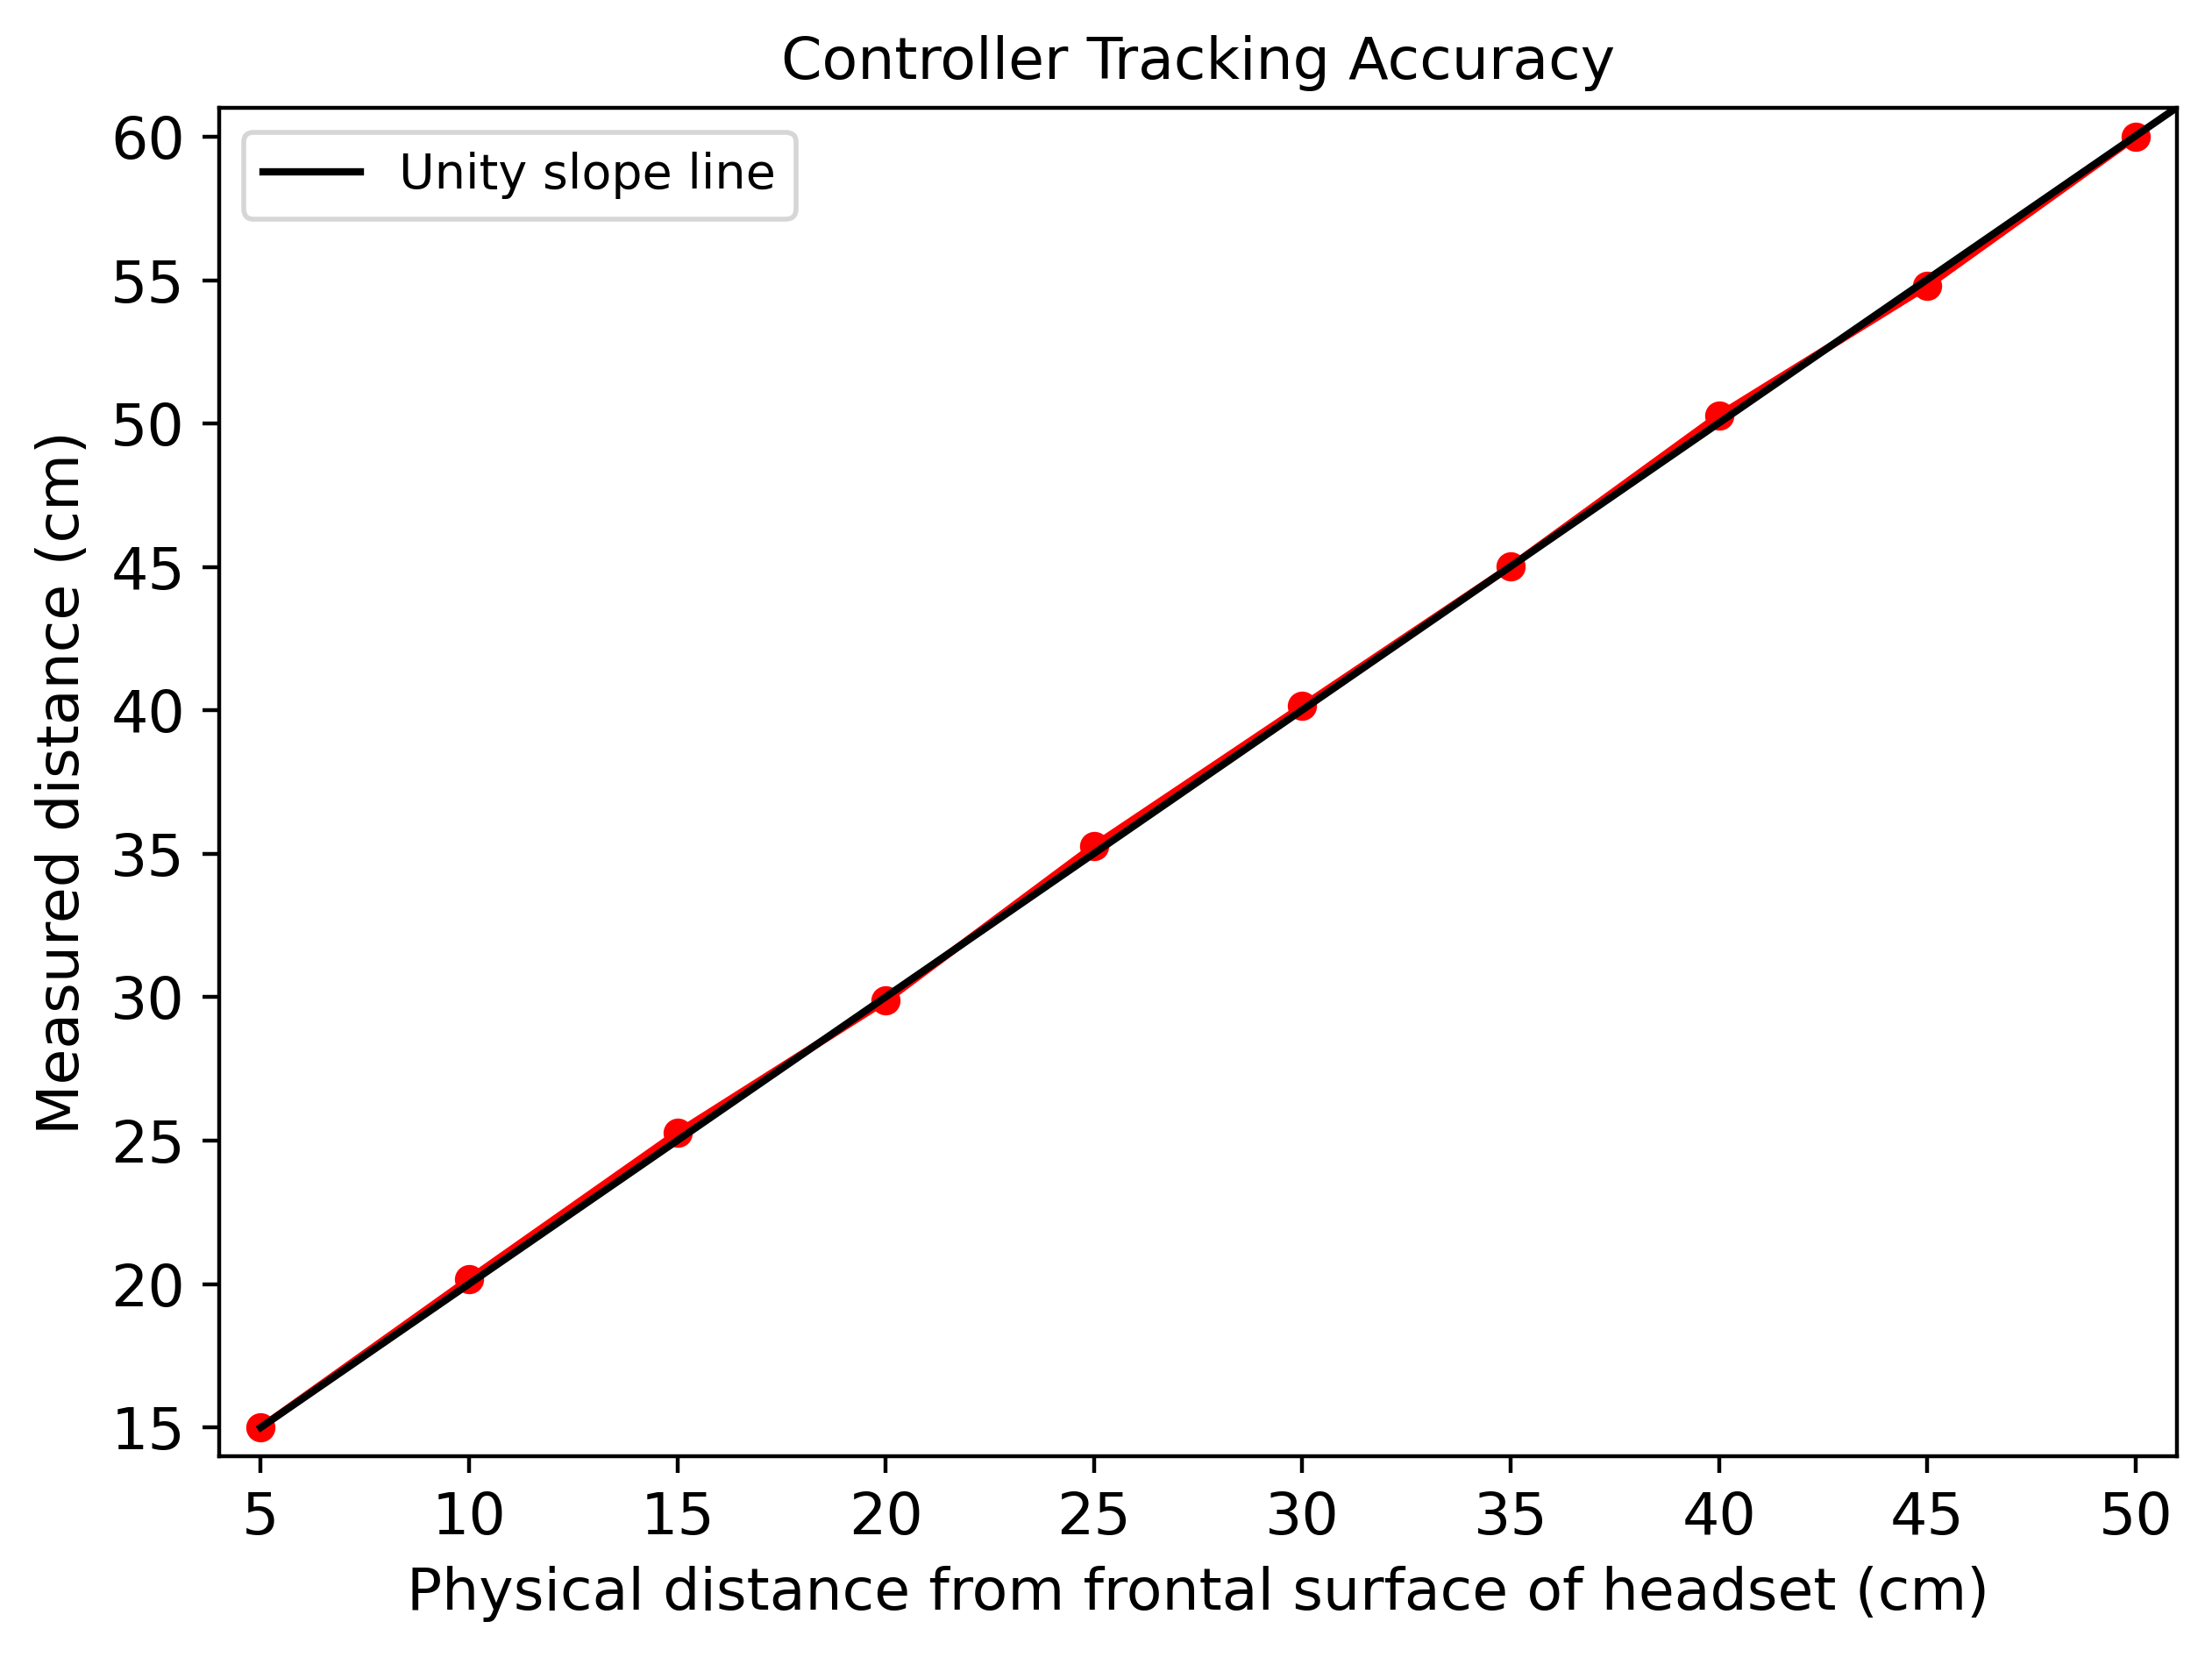
\includegraphics[width=.7\textwidth]{figures/supplement/suppl_controller_tracking_accuracy_plot.png}
	\caption{Relationship between tracked controller distance and physical distance from the frontal surface of the Quest 3.  }
	\label{fig:suppl_controller_tracking_accuracy_plot}
\end{figure}

\FloatBarrier
\newpage

\section{Algorithm for Simulating Rendering and Viewing Errors in Unity}

\FloatBarrier

\hspace{12pt}Step 1: 
\begin{figure}[h]
	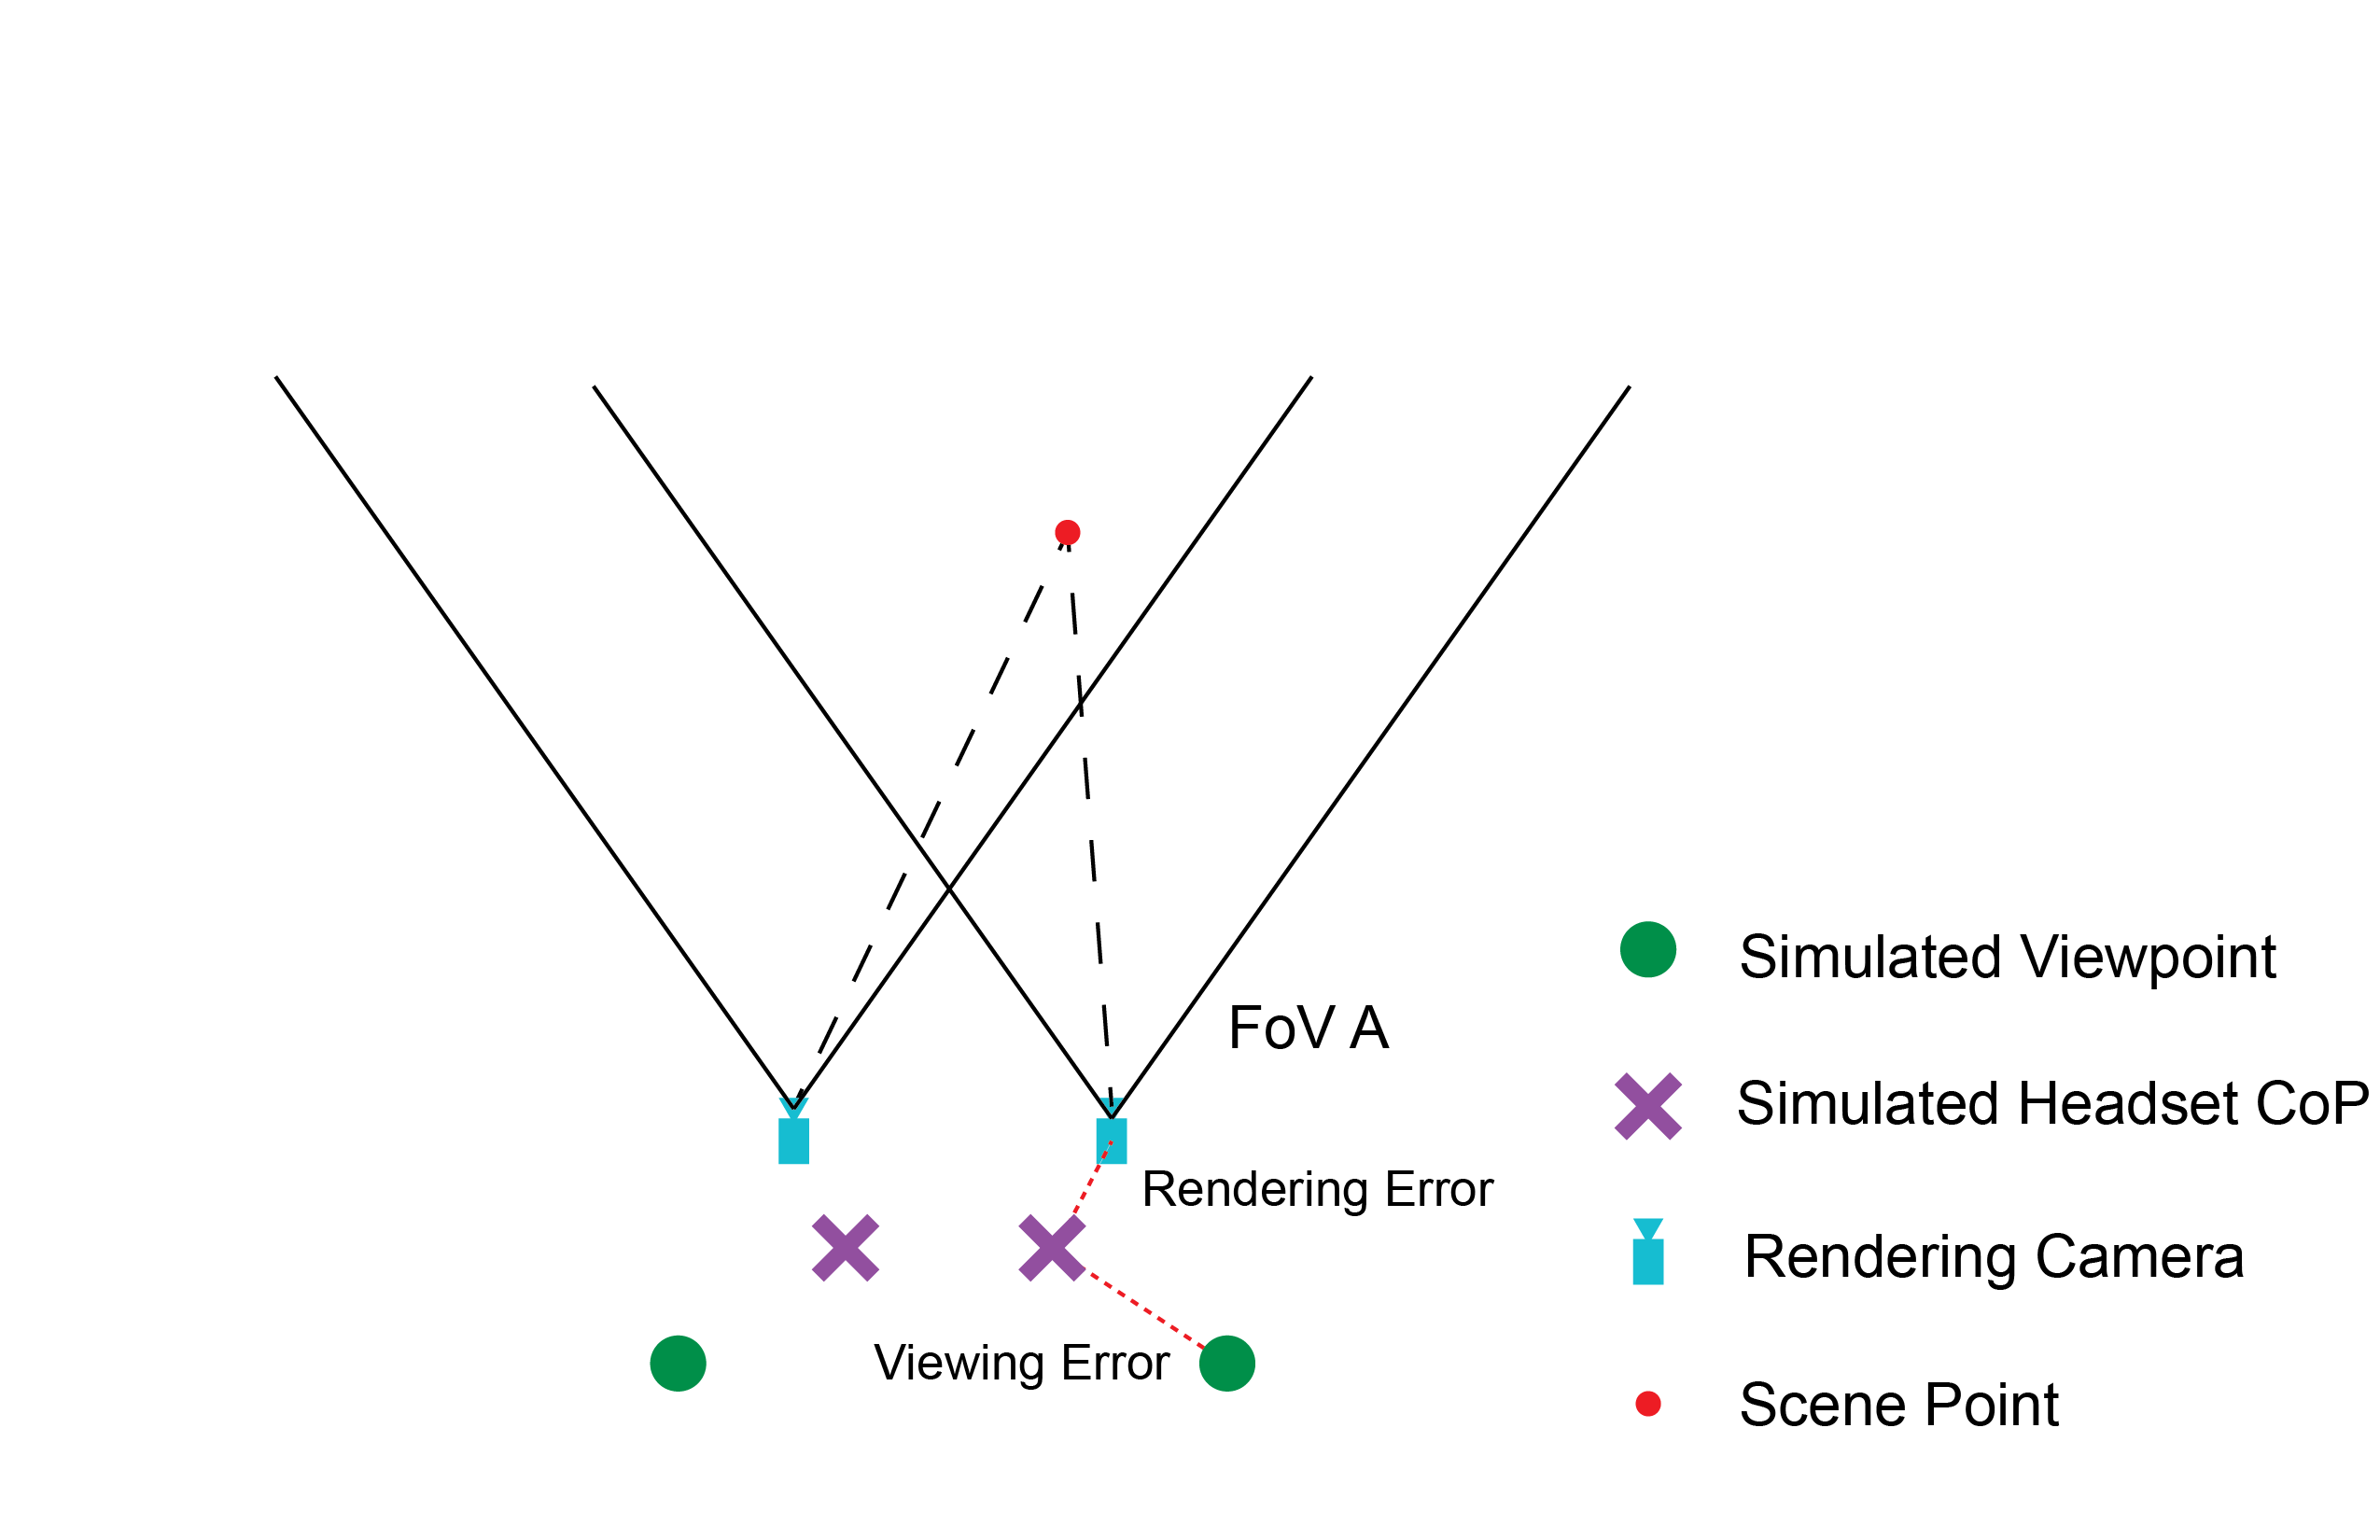
\includegraphics[width=0.65\textwidth]{figures/supplement/unity/1.png}
	\caption{Rendering camera renders the scene with field of view (FoV) A. Rendering error is the displacement of rendering camera from headset Center of Projection (CoP). }
	\label{fig:unity/1}
\end{figure}

\FloatBarrier

\FloatBarrier
Step 2: 
\begin{figure}[h]
	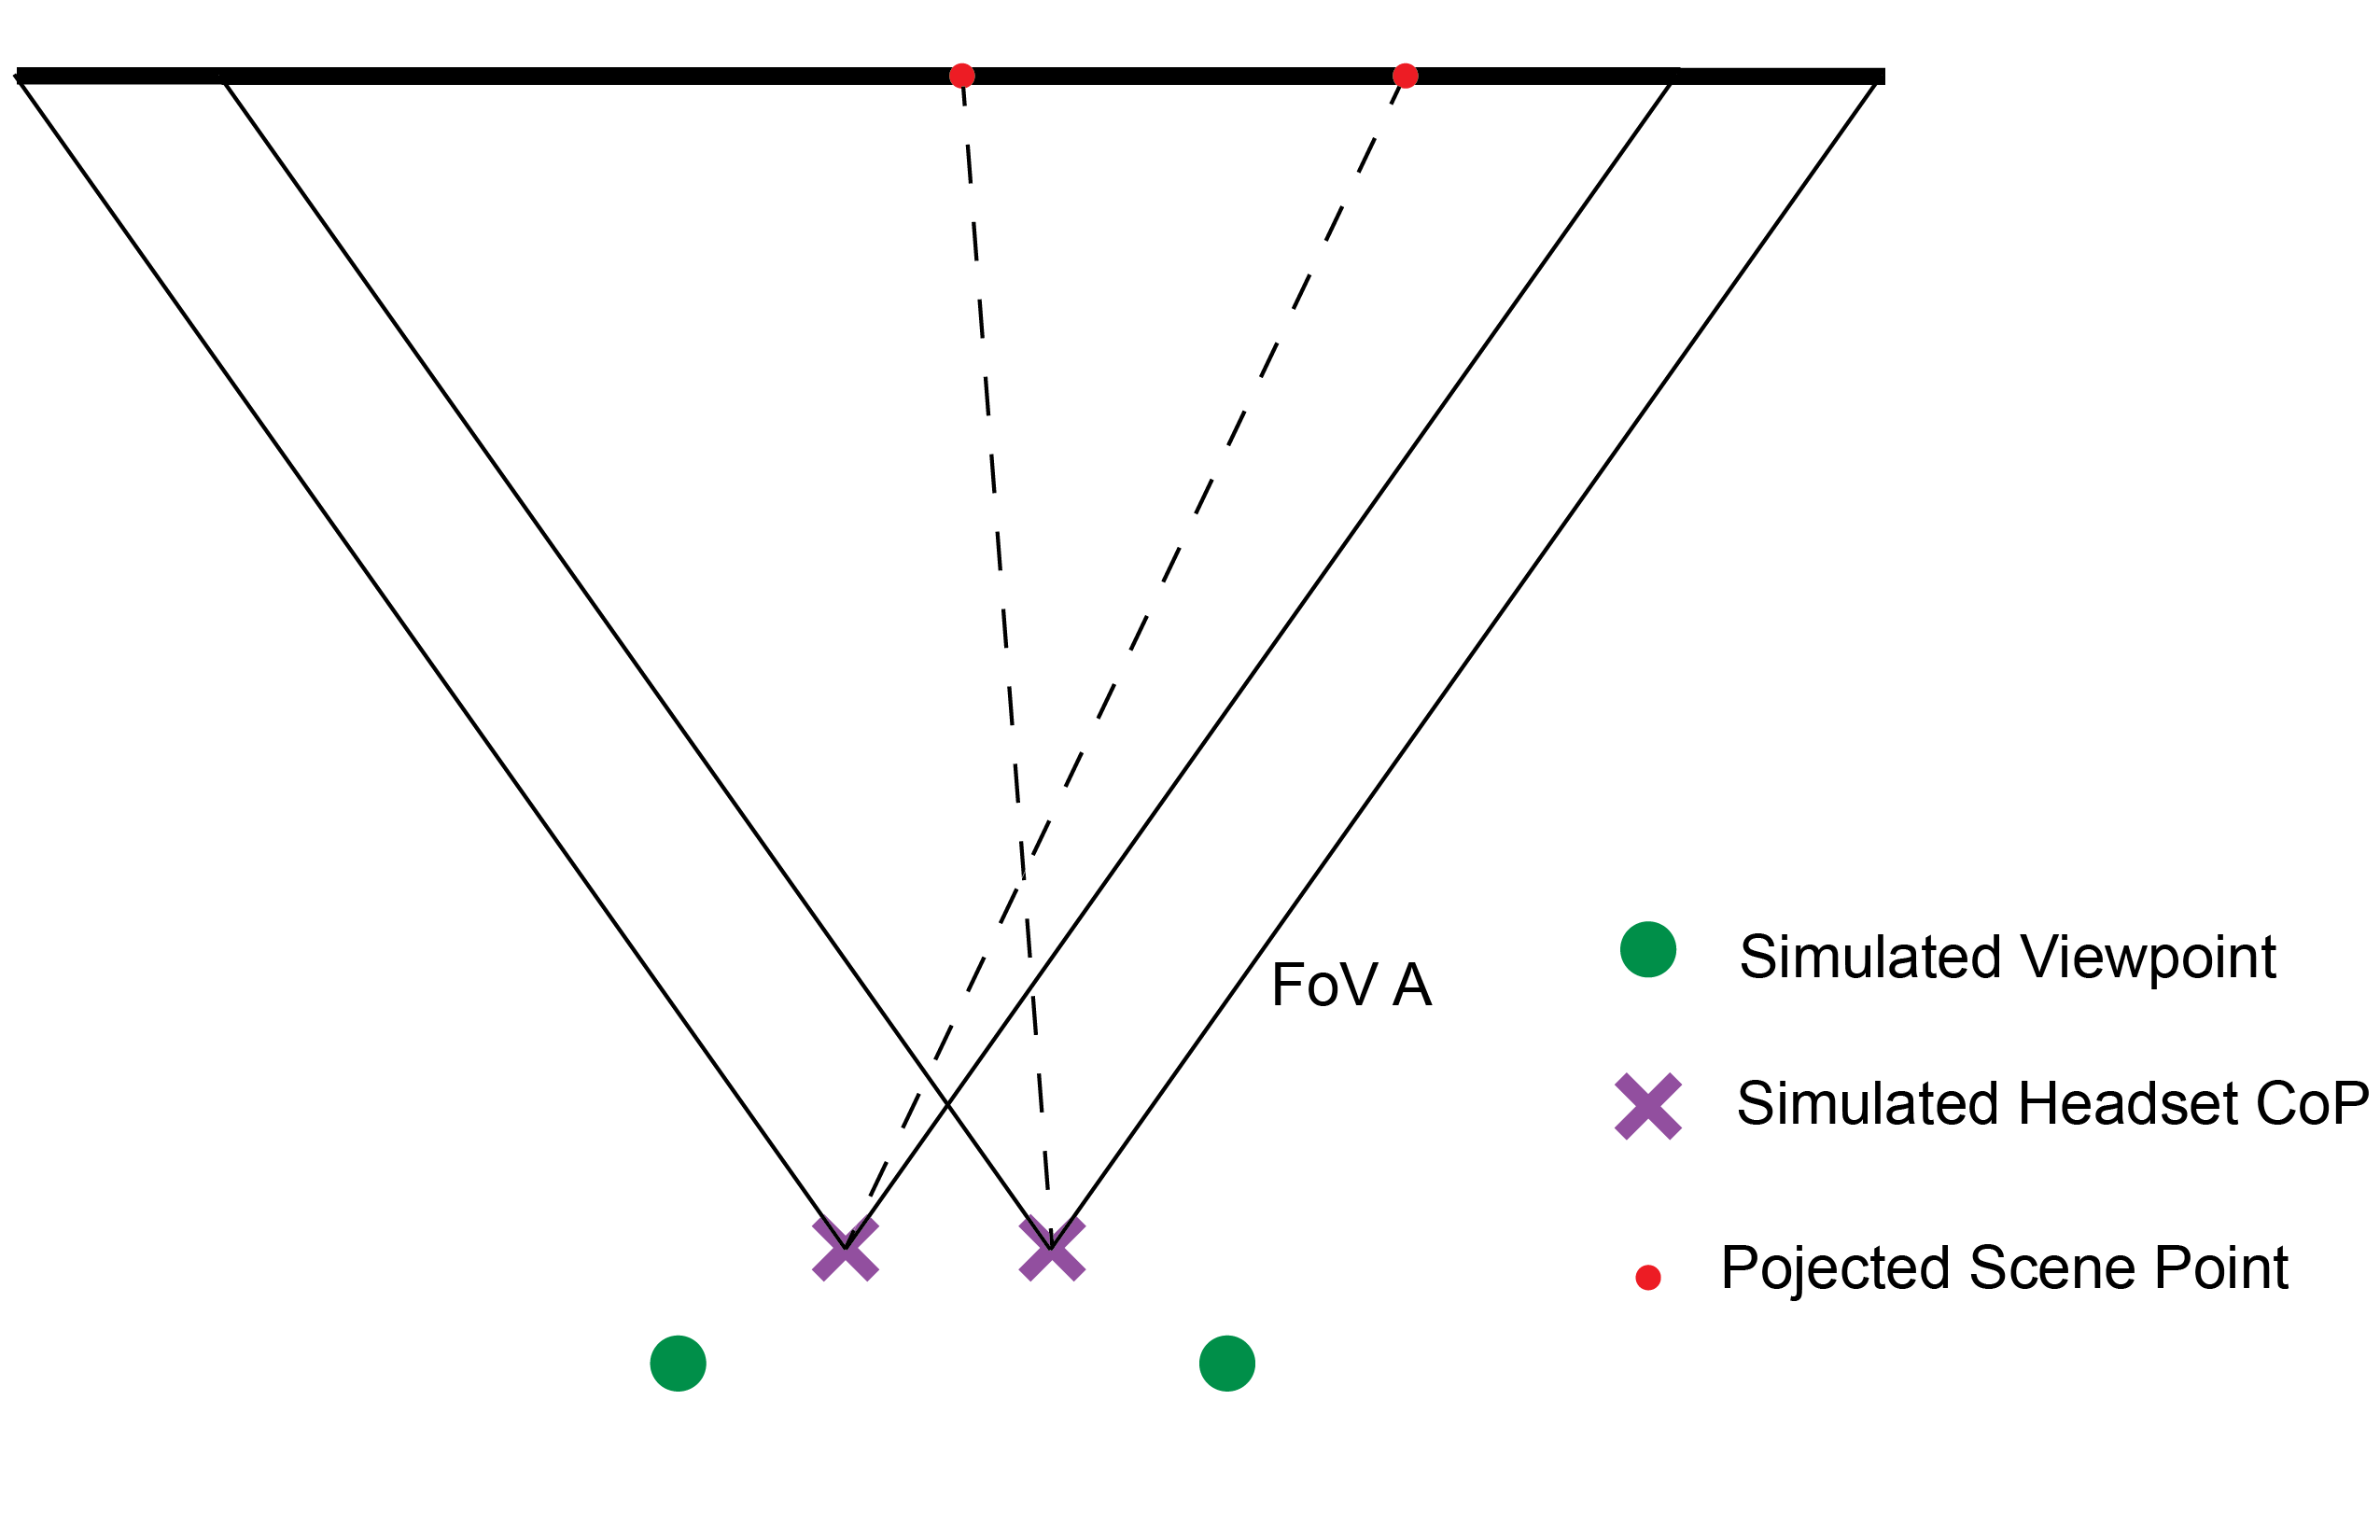
\includegraphics[width=0.65\textwidth]{figures/supplement/unity/2.png}
	\caption{Frame buffer of rendering camera is projected to a quad at the same plane as the virtual image plane. The quad size matches FoV A.}
	\label{fig:unity/2}
\end{figure}

\FloatBarrier
\newpage

\FloatBarrier
Step 3: 
\begin{figure}[h]
	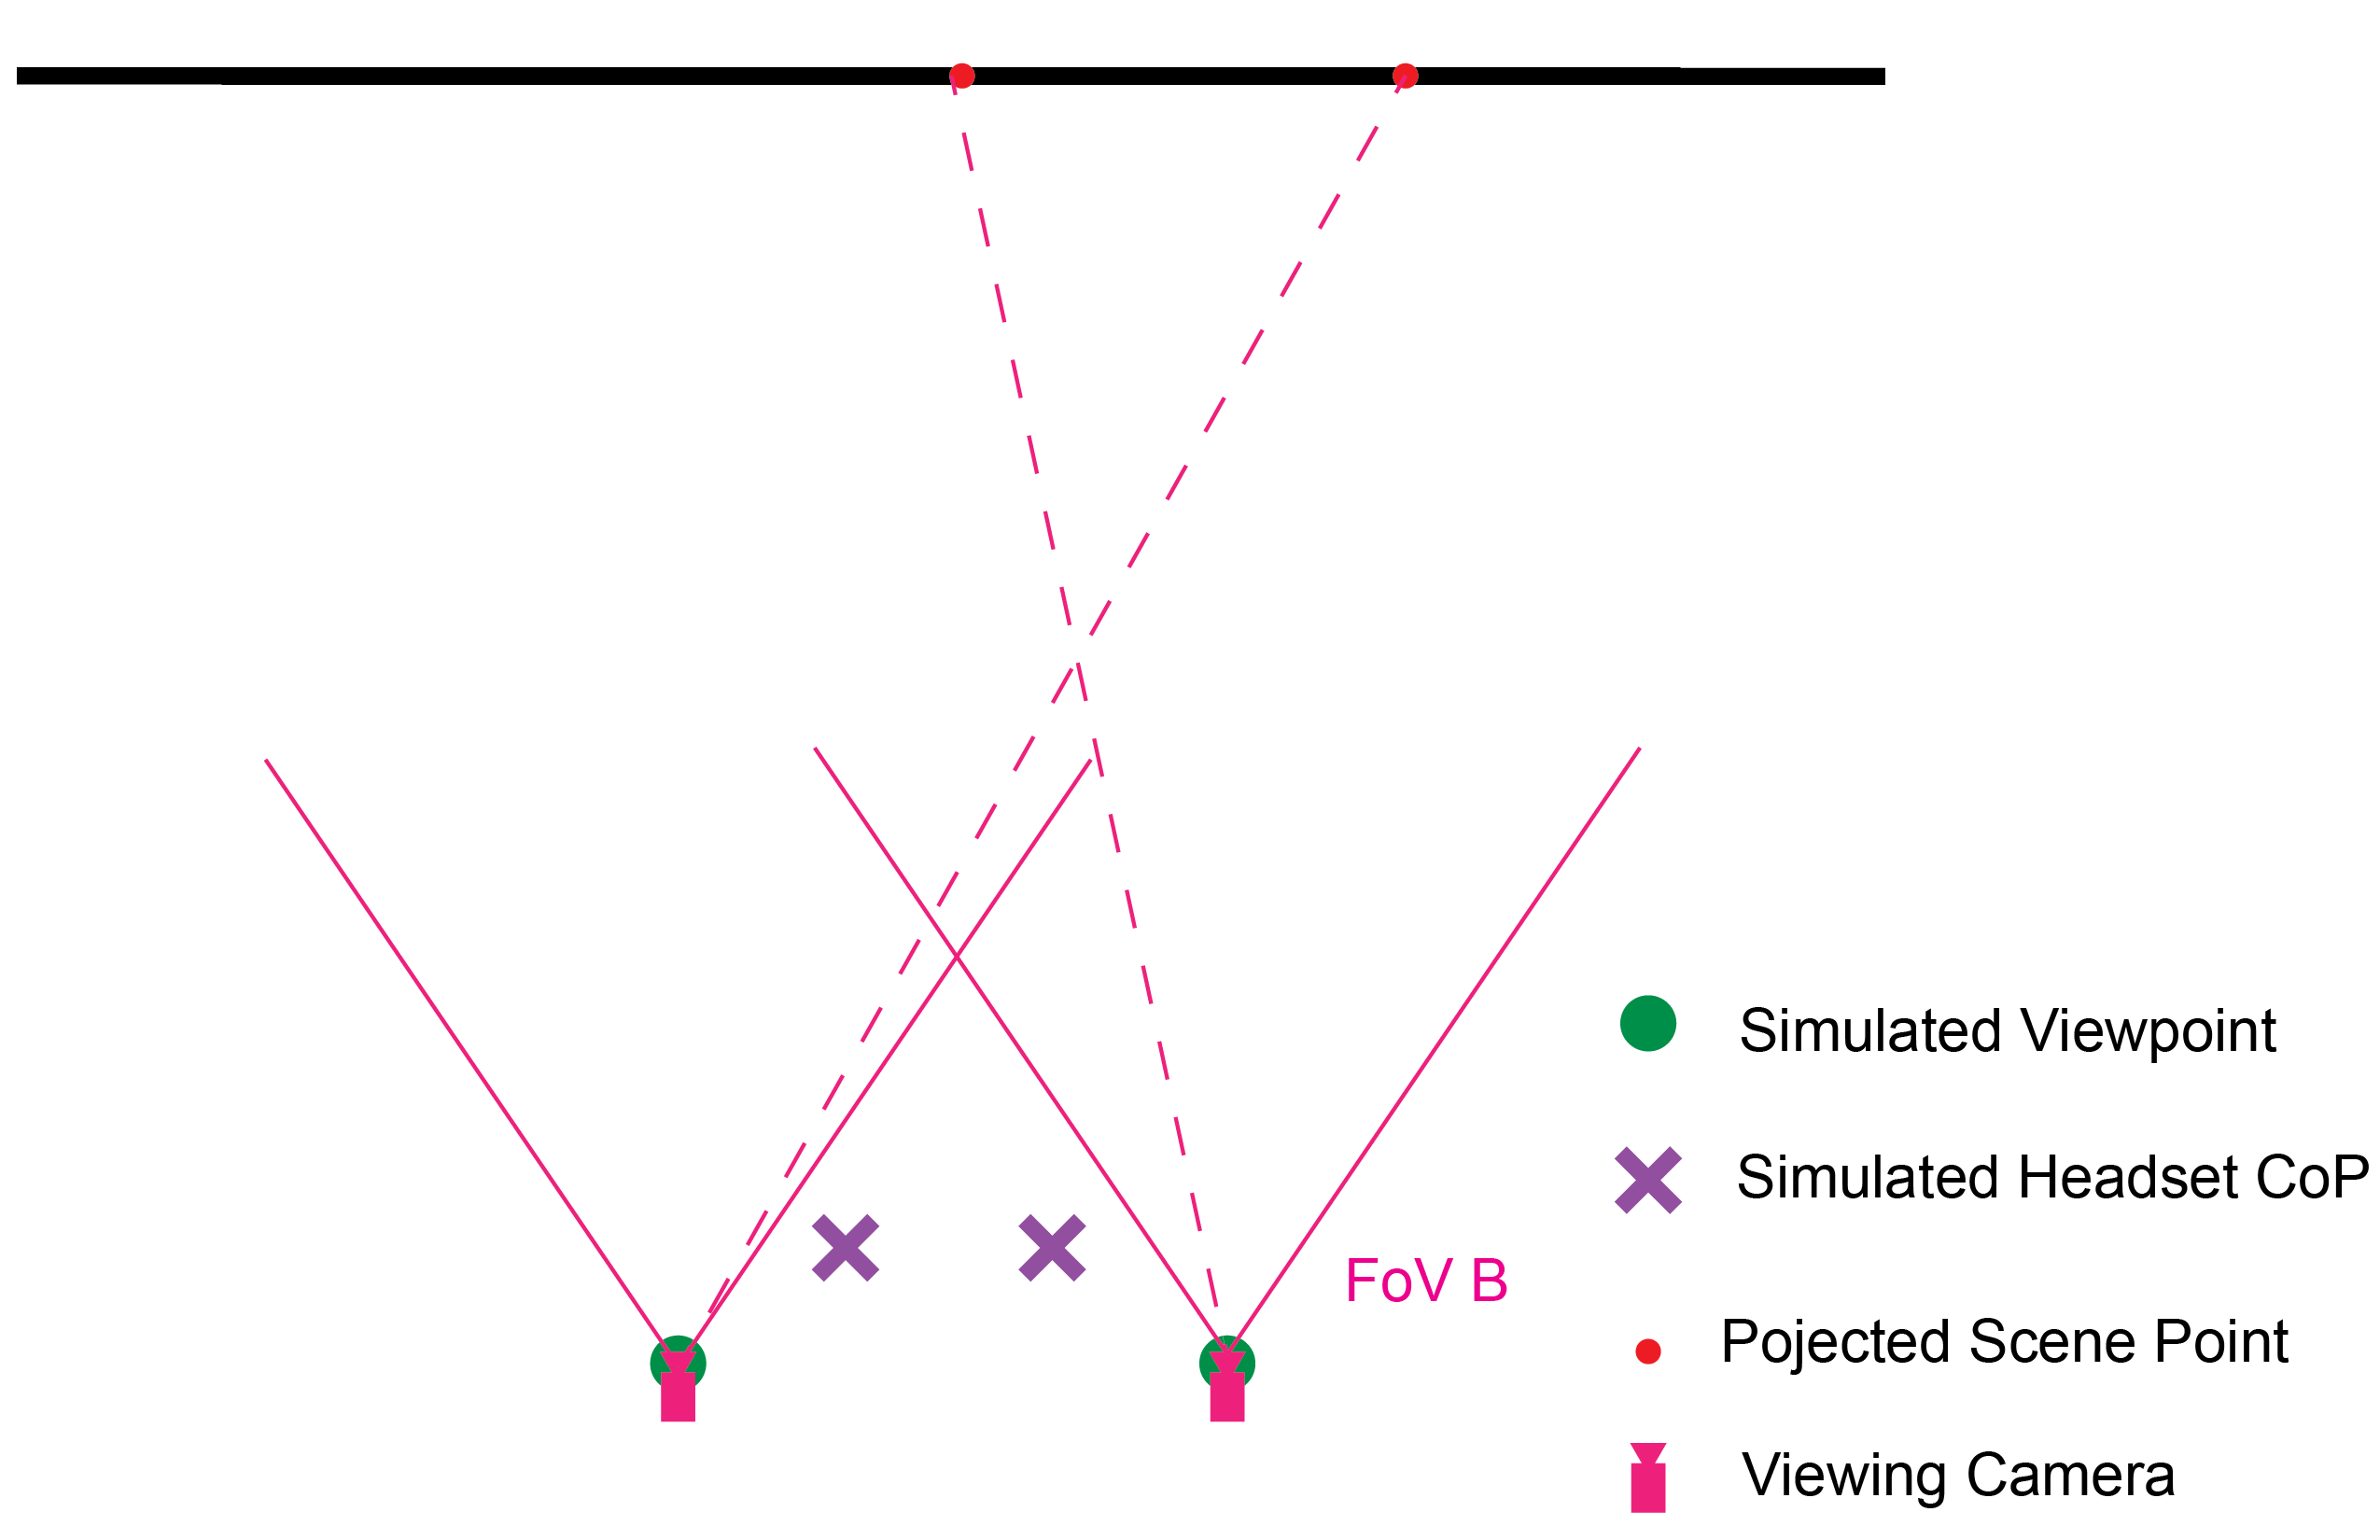
\includegraphics[width=0.65\textwidth]{figures/supplement/unity/3.png}
	\caption{Viewing camera with FoV B views this quad from the simulated viewpoint. Viewing error is the displacement of simulated user CoP from headset CoP. At parallel gaze, simulated user CoP coincides with simulated viewpoint.}
	\label{fig:unity/3}
\end{figure}

\FloatBarrier

\FloatBarrier
Step 4: 
\begin{figure}[h]
	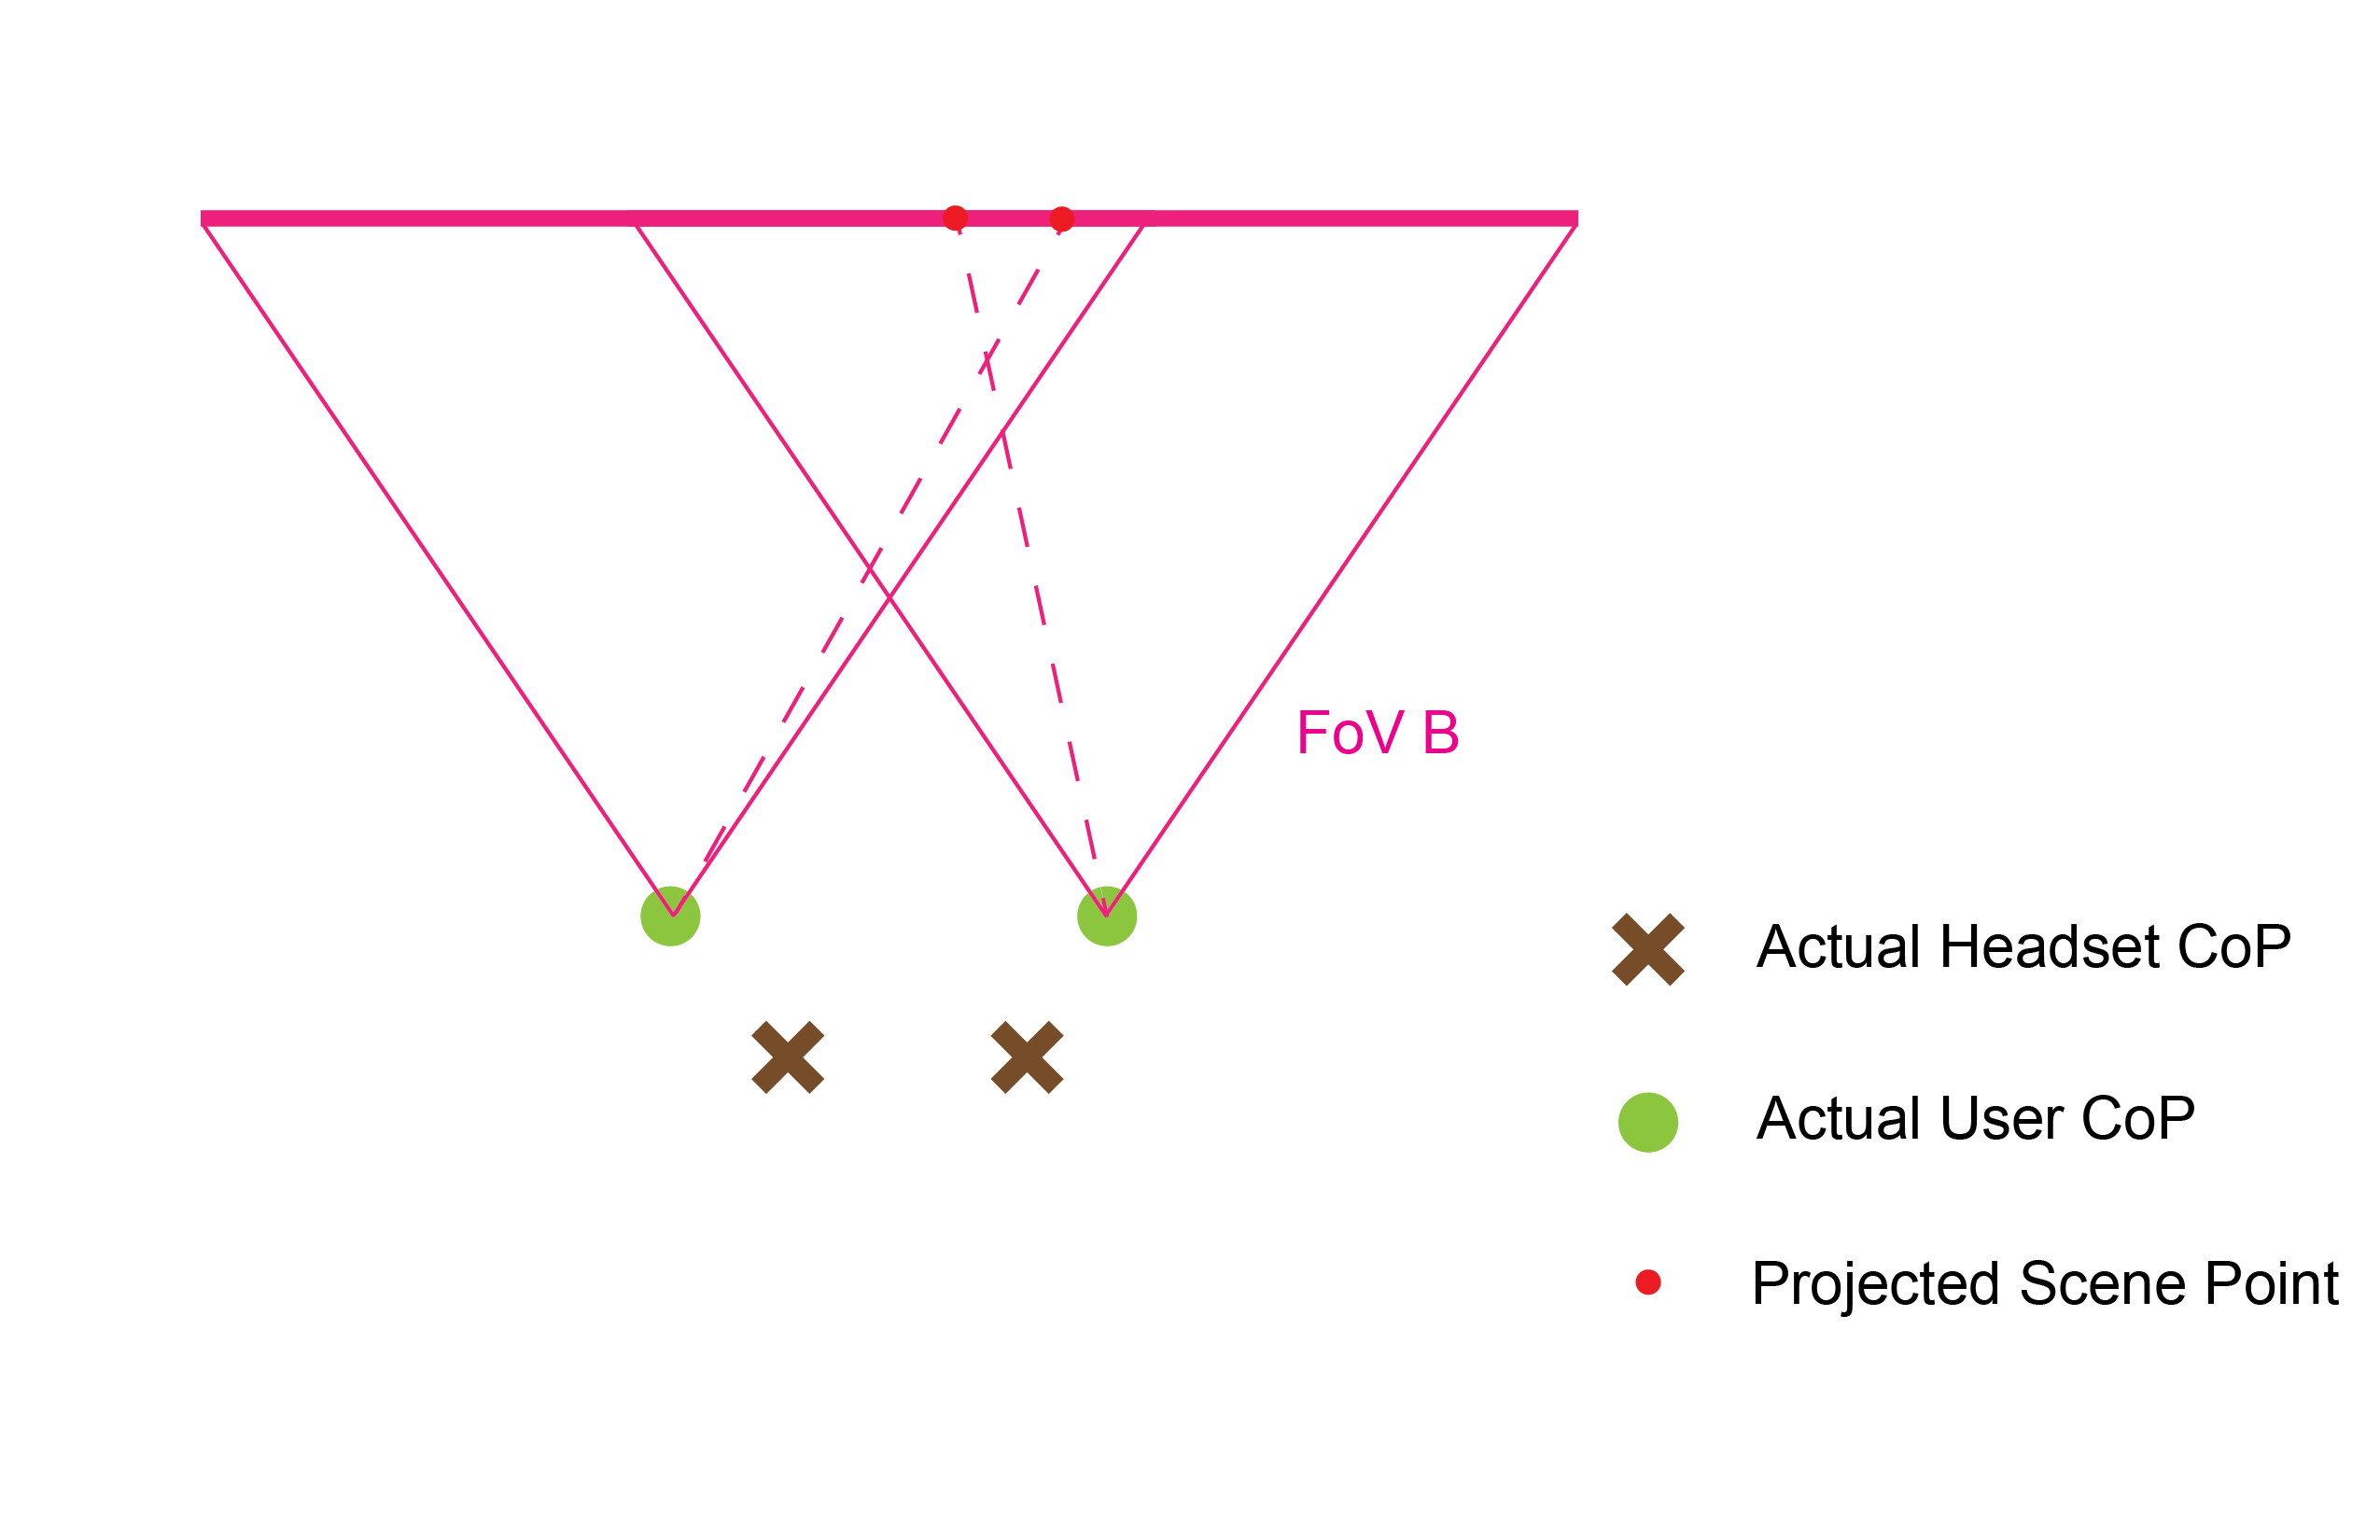
\includegraphics[width=0.65\textwidth]{figures/supplement/unity/4.png}
	\caption{Frame buffer of viewing camera is projected from the actual user CoP position to a quad. The quad size matches FoV B. We used tracked entrance pupil position to approximate actual user CoP position.}
	\label{fig:unity/4}
\end{figure}

\FloatBarrier
\newpage
\FloatBarrier
Step 5: 
\begin{figure}[h]
	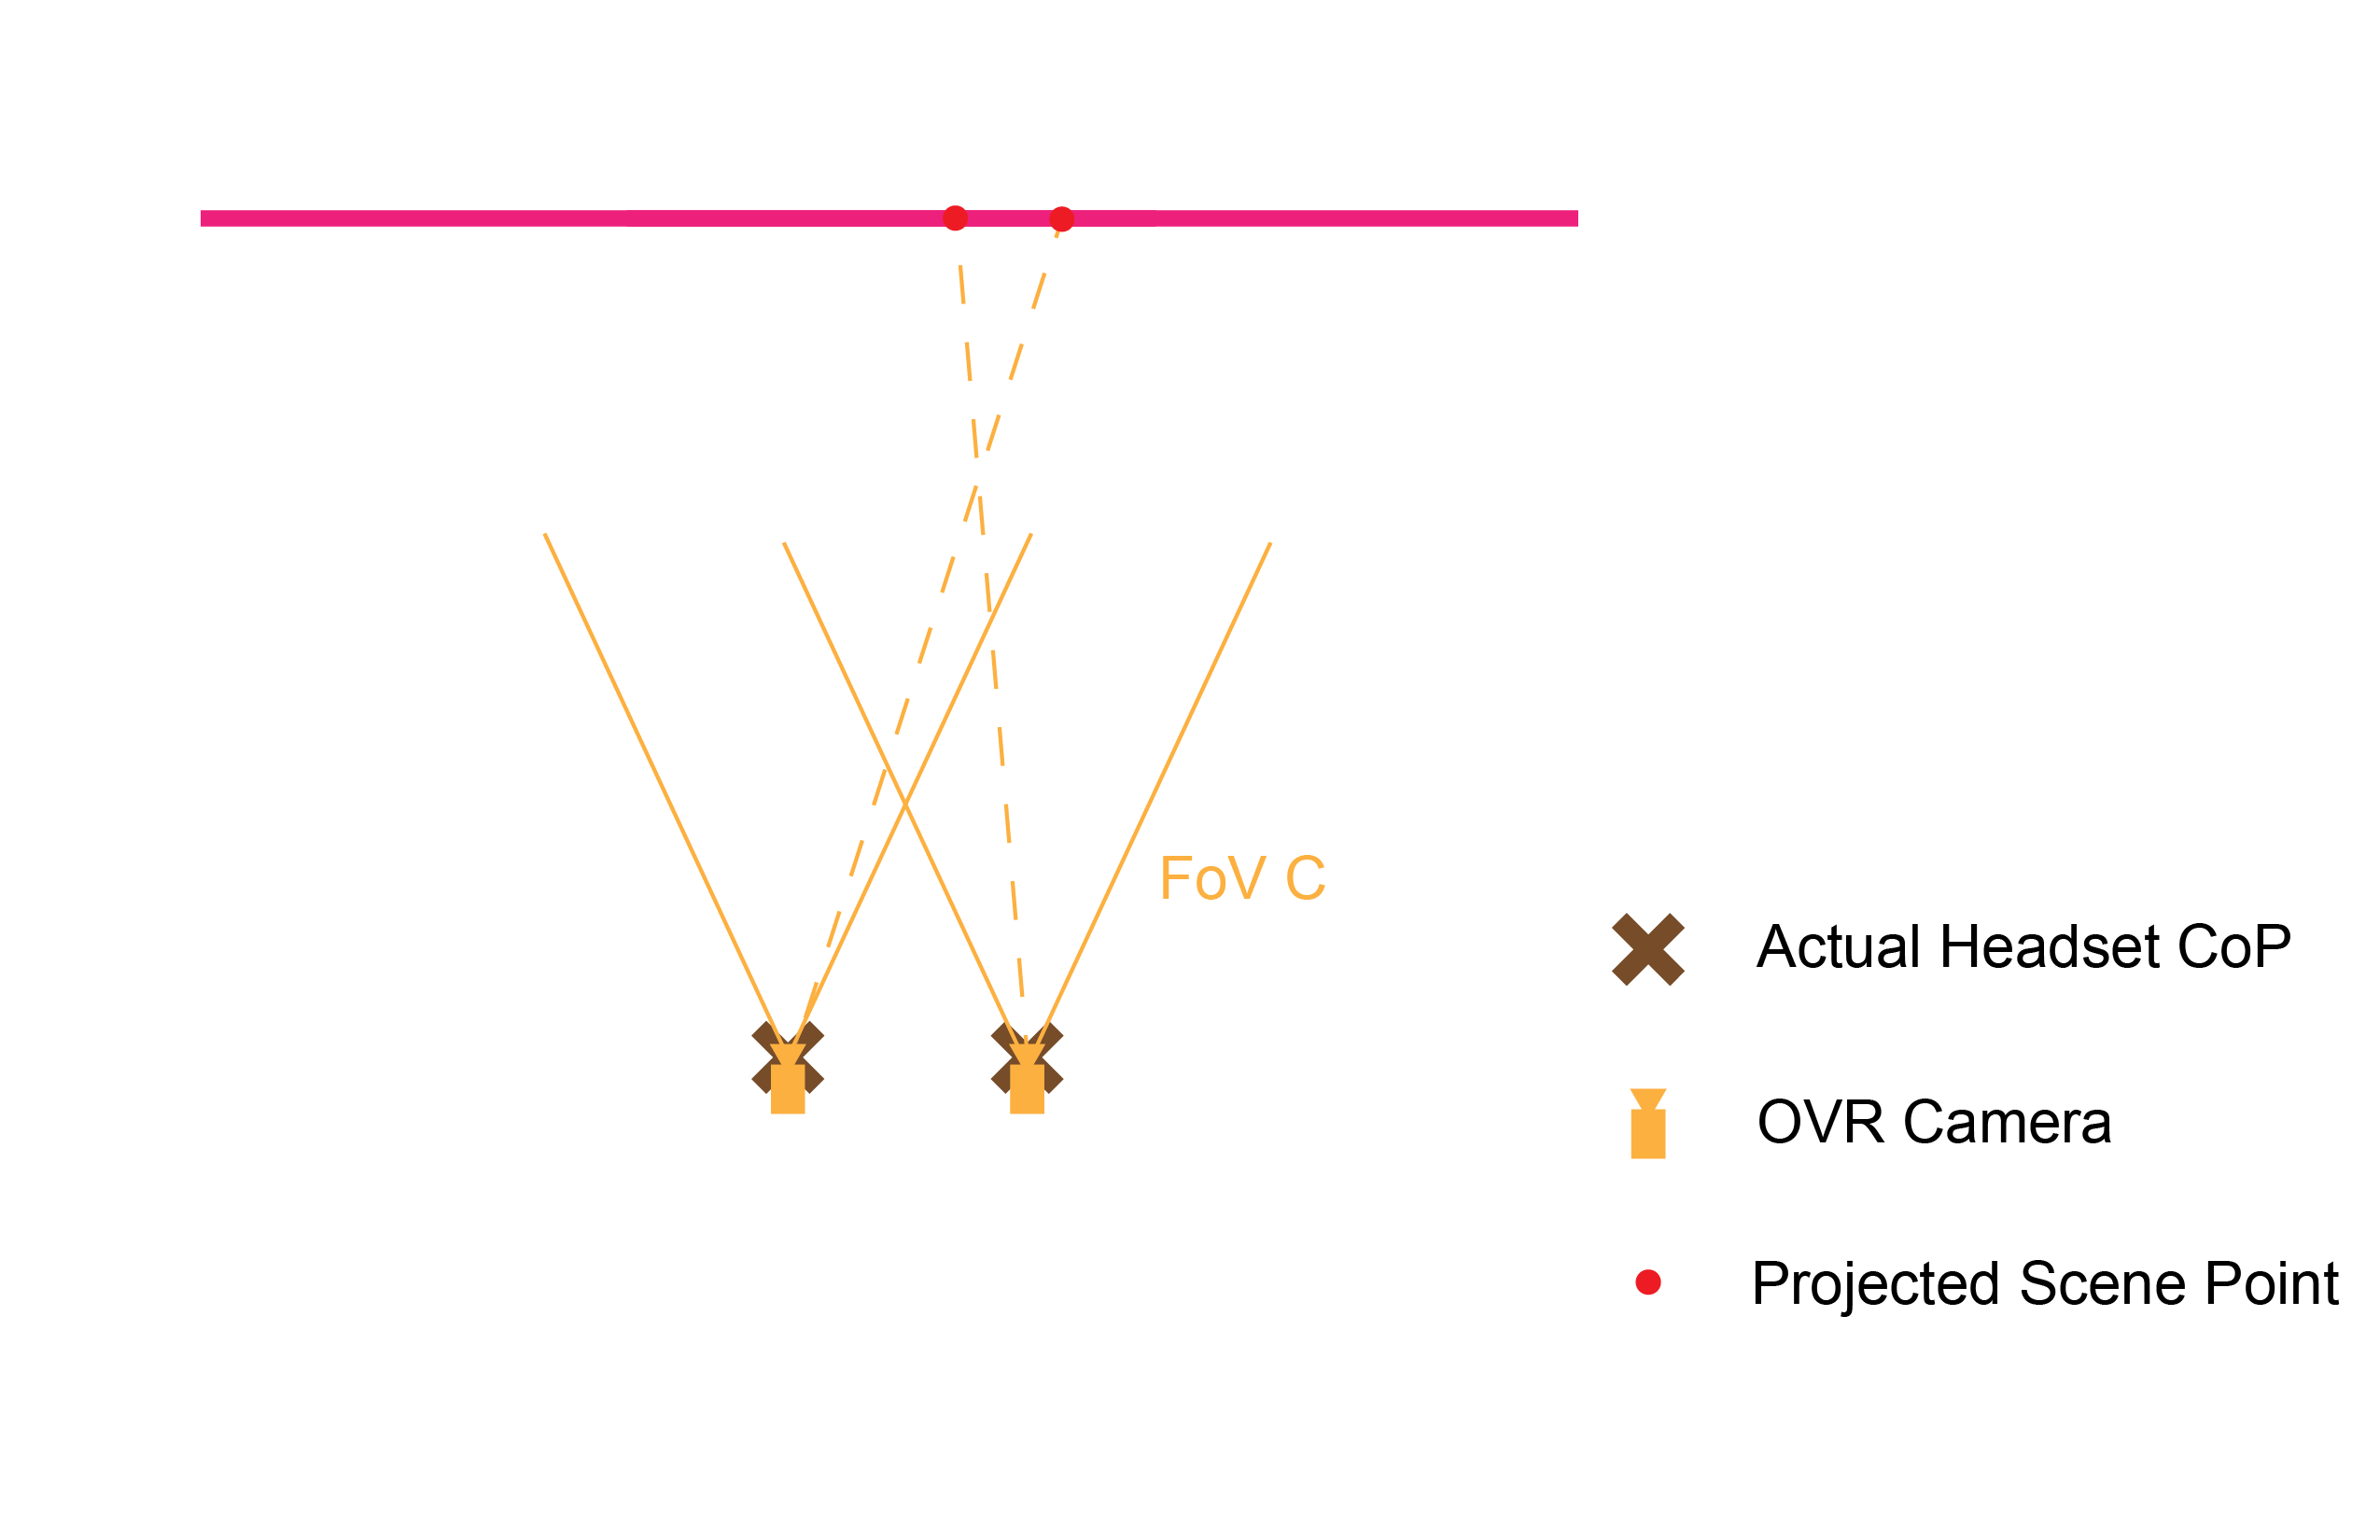
\includegraphics[width=0.65\textwidth]{figures/supplement/unity/5.png}
	\caption{The OVR camera subsequently views this quad and sends its frame buffer to the actual headset display.}
	\label{fig:unity/5}
\end{figure}
\FloatBarrier

\bibliographystyle{ACM-Reference-Format}
\bibliography{bib}	

\end{document}